\subsection{Occlusion and ID Switching Analysis}

For visualization clarity, all frame sequences shown in this subsection are cropped and magnified from the original high-resolution video.

\subsubsection{Dynamic Target Interaction: Pedestrian Crossing}

Figure~\ref{fig:pedestrian_cross} shows a short-term interaction scenario where two pedestrians cross each other at close range. In Frame~304, both pedestrians are successfully tracked with IDs 9759 and 11824. In Frame~305, the two targets heavily overlap, causing both tracking IDs to disappear temporarily. During Frames~305--306, the detector fails to output stable bounding boxes for either pedestrian.

The primary reason for this failure is that the two small-scale pedestrians become visually merged during overlap. As a result, the detector confidence decreases significantly, and the detector can no longer reliably separate the two targets into independent detections. Since ByteTrack relies on detector outputs as the basis for association, the disappearance of valid detections directly interrupts the corresponding tracks.

When the pedestrians begin separating again in Frame~307, one tracking ID (11824) is successfully recovered. By Frame~308, both IDs are restored, and the tracker reassociates the pedestrians with their original identities instead of assigning new IDs.

\begin{figure}[htbp]
    \centering
    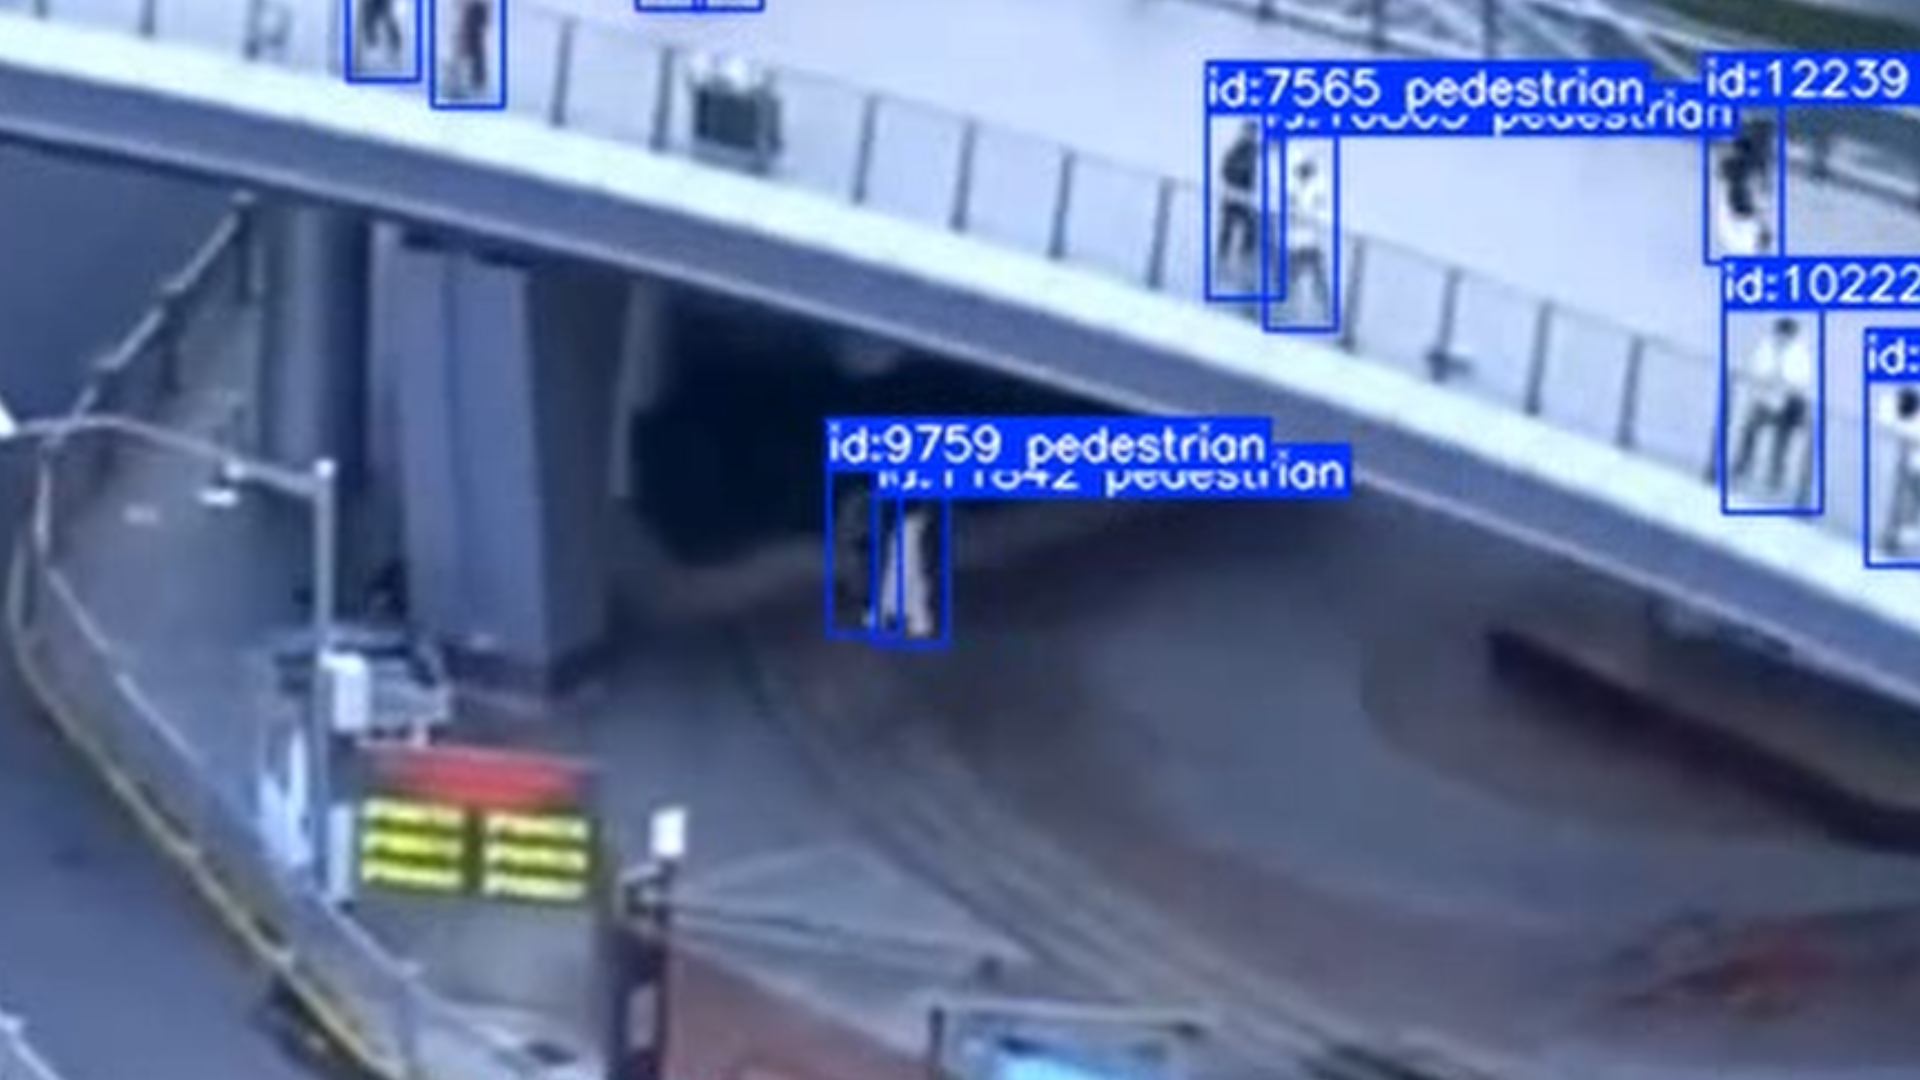
\includegraphics[width=0.19\textwidth]{figures/task2/Frames/Frame 304.jpg}
    \hfill
    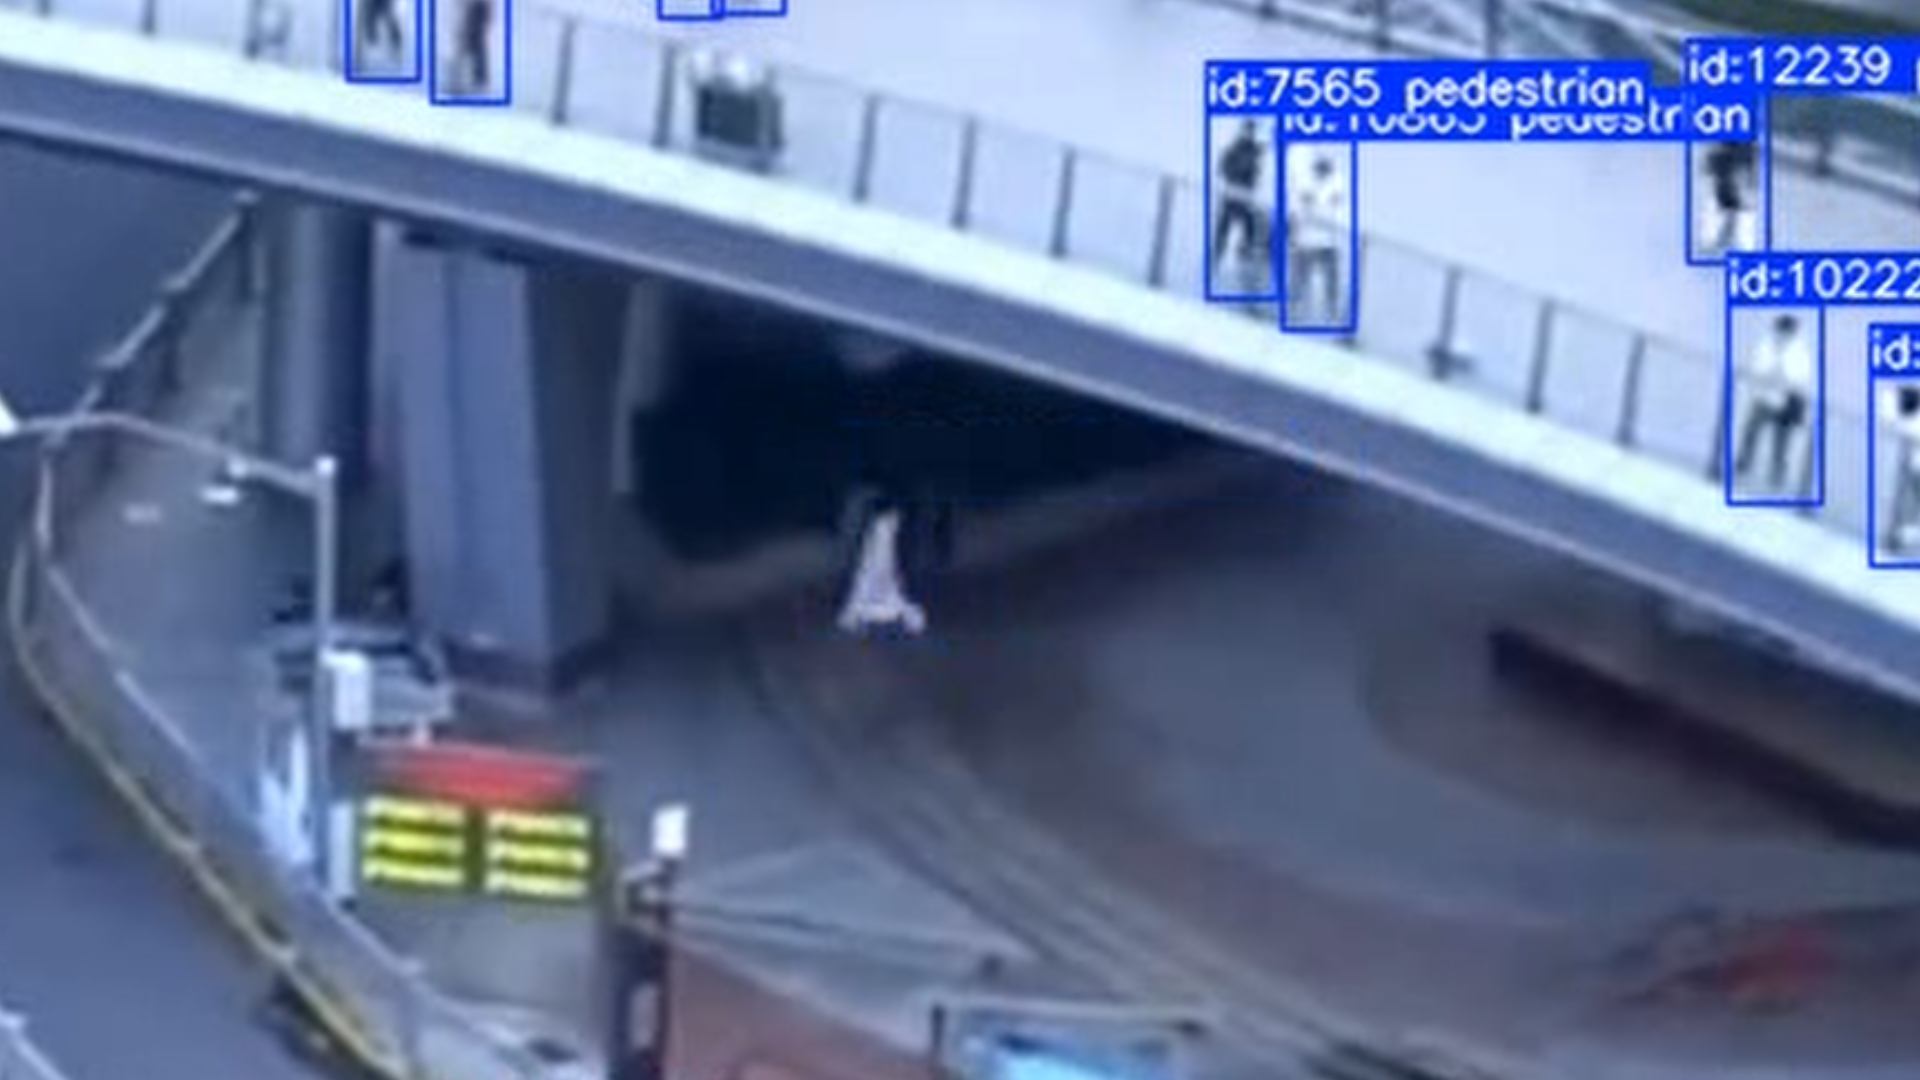
\includegraphics[width=0.19\textwidth]{figures/task2/Frames/Frame 305.jpg}
    \hfill
    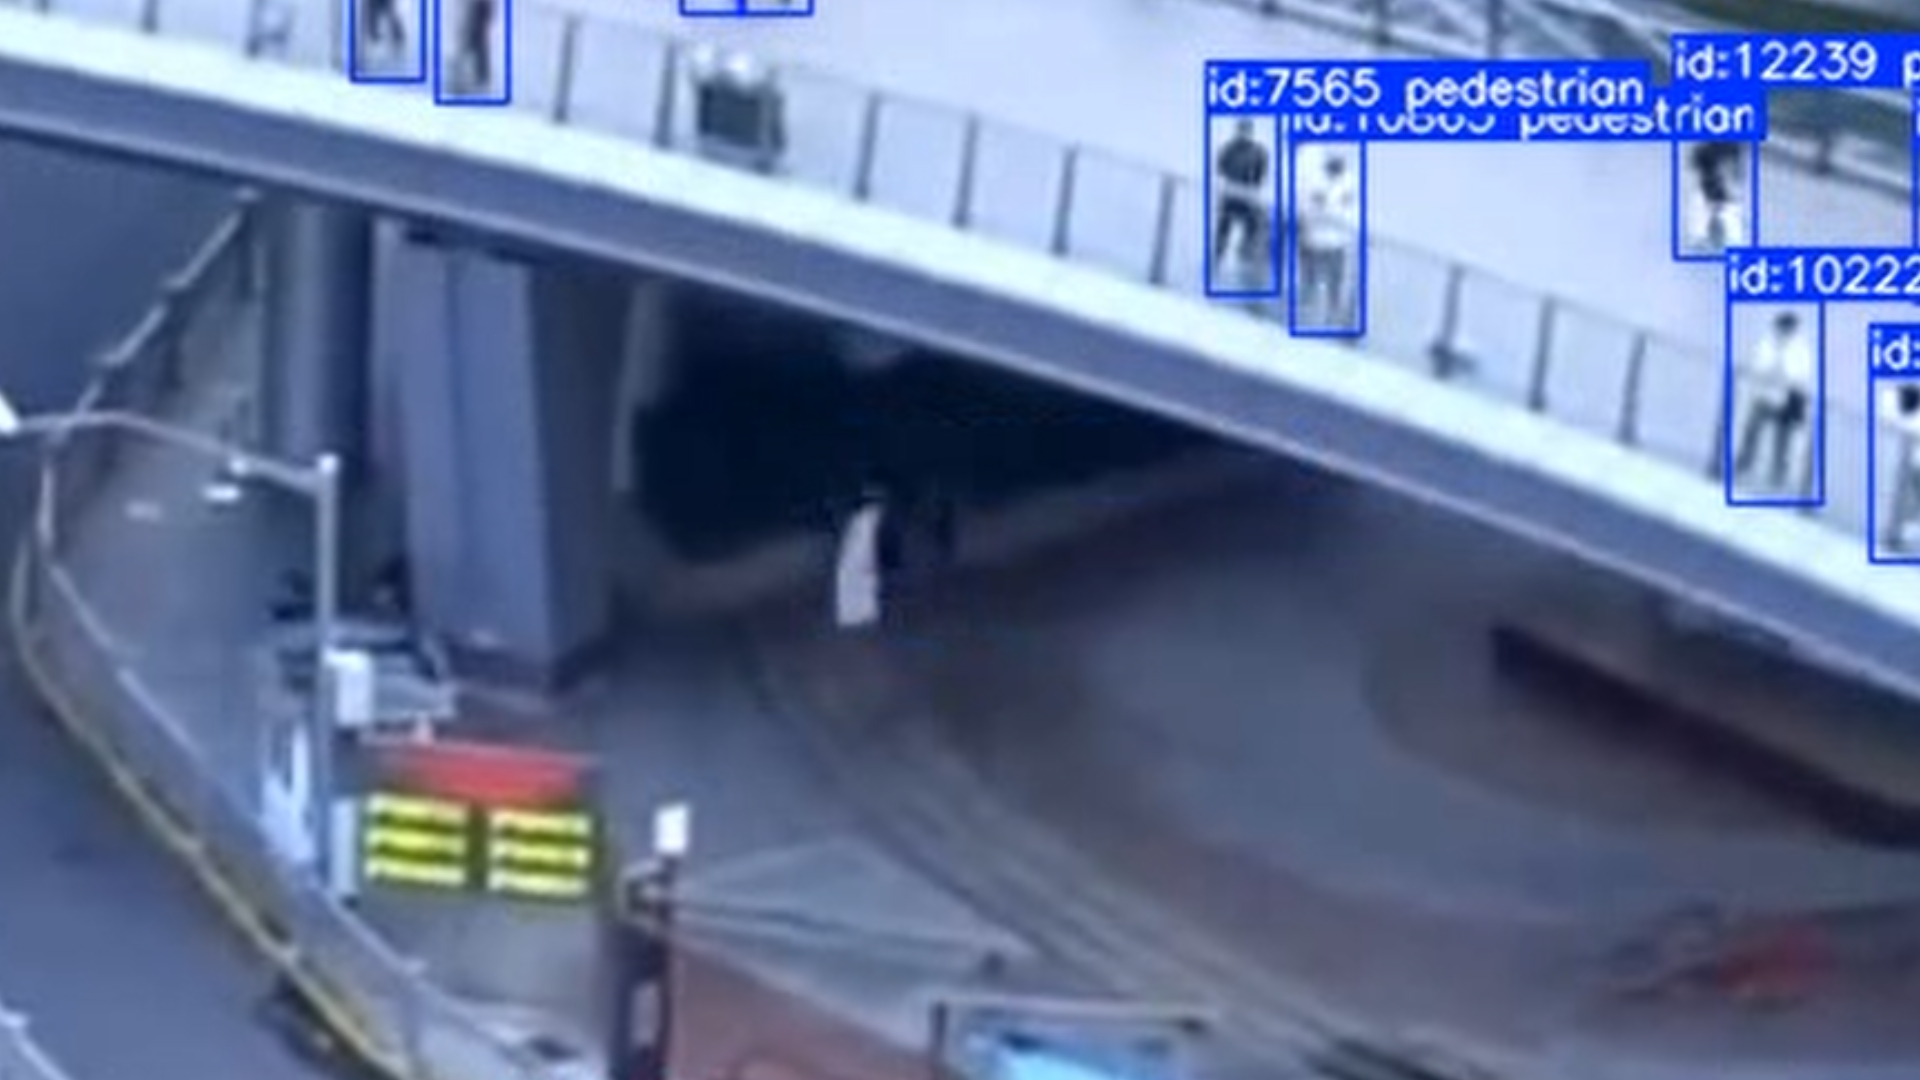
\includegraphics[width=0.19\textwidth]{figures/task2/Frames/Frame 306.jpg}
    \hfill
    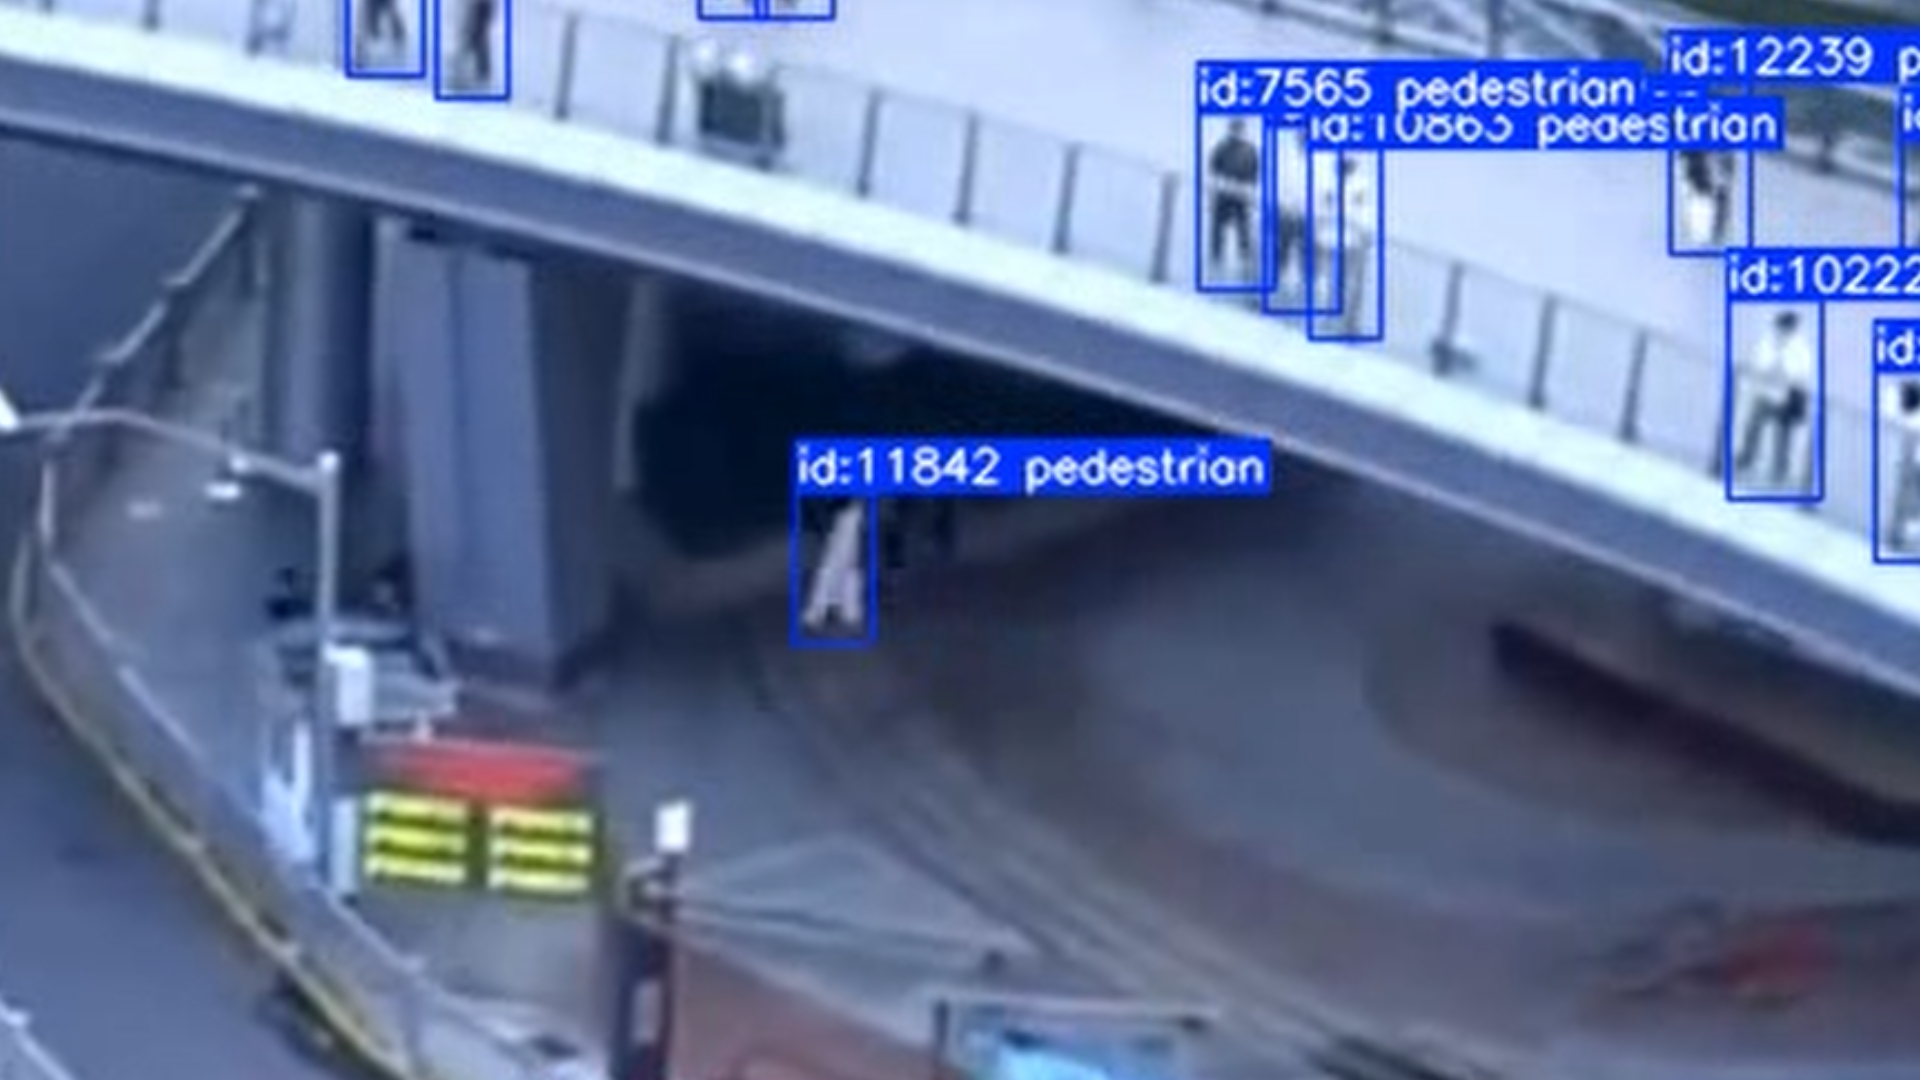
\includegraphics[width=0.19\textwidth]{figures/task2/Frames/Frame 307.jpg}
    \hfill
    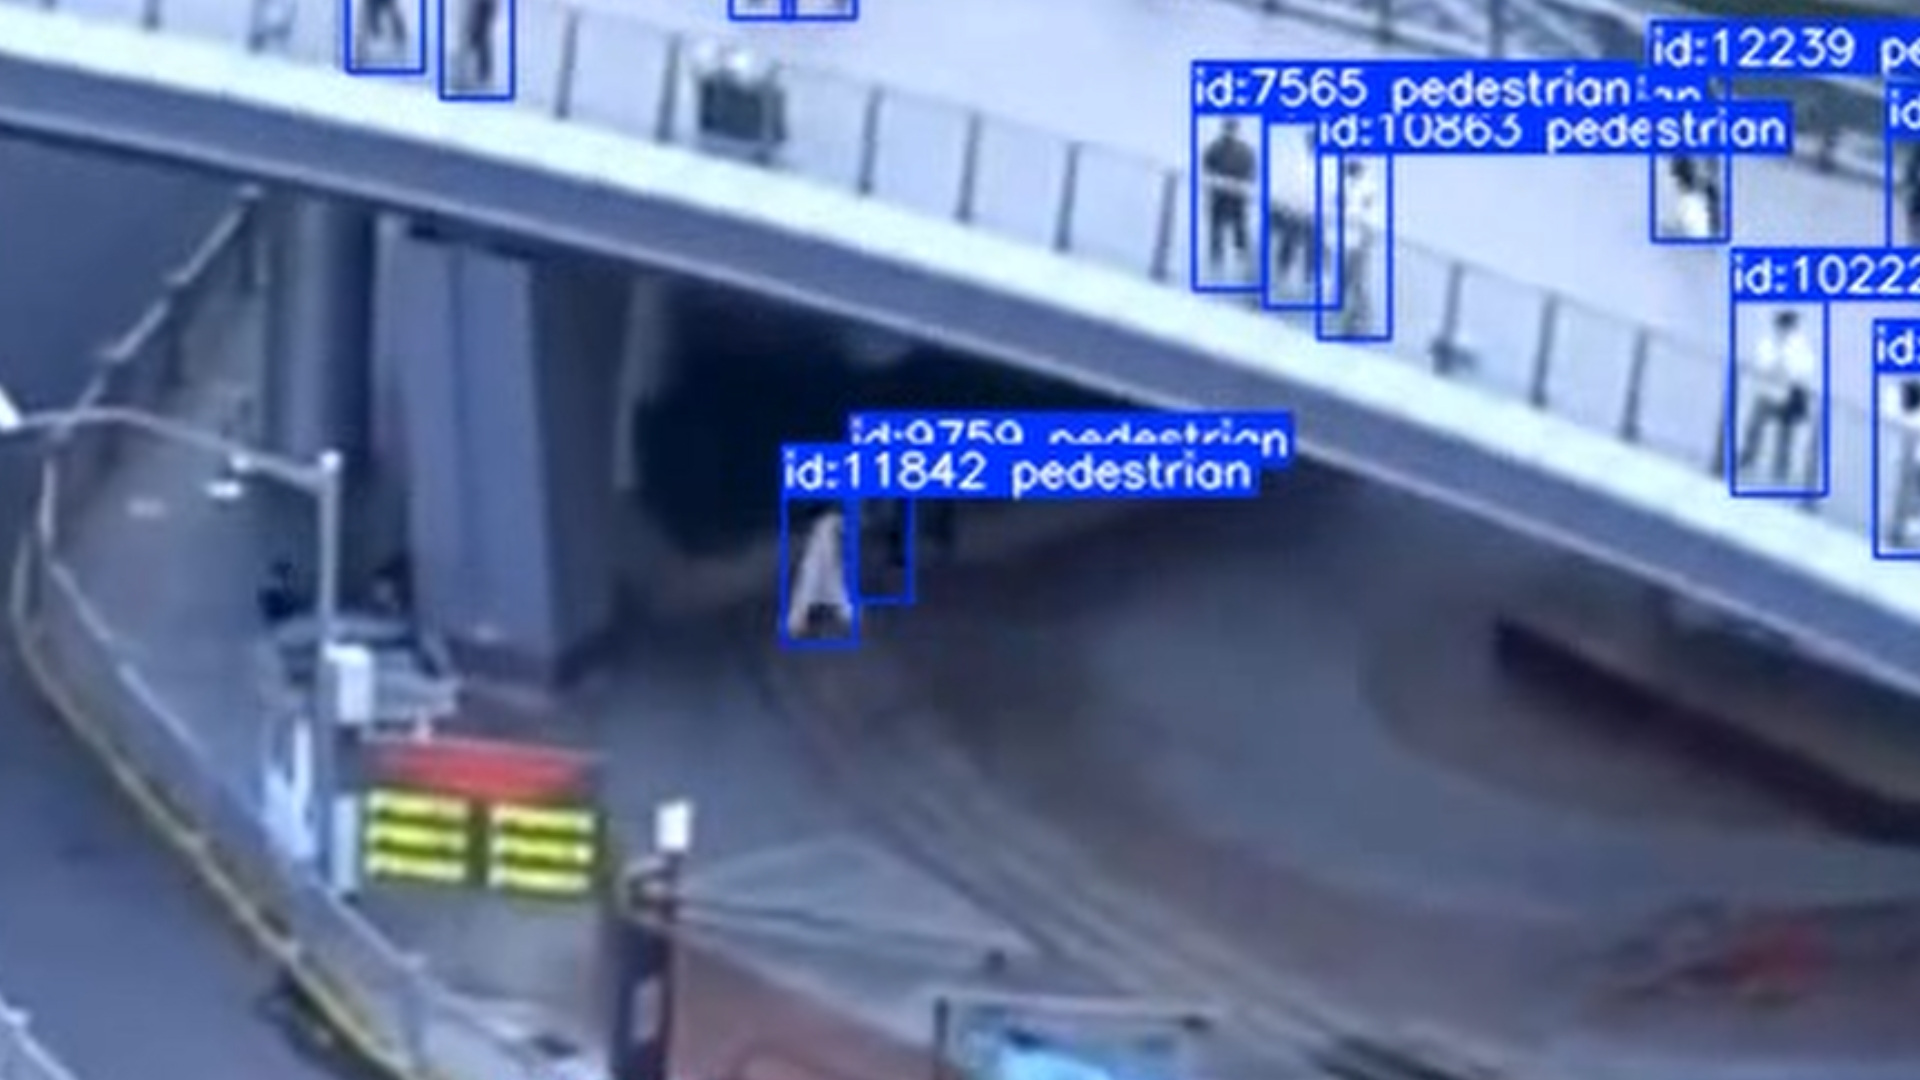
\includegraphics[width=0.19\textwidth]{figures/task2/Frames/Frame 308.jpg}

    \vspace{0.3em}
    {\hspace{0.05\linewidth}\small Frame 304 \hfill Frame 305 \hfill Frame 306 \hfill Frame 307 \hfill Frame 308\hspace{0.05\linewidth}}

    \caption{Pedestrian crossing scenario with short-term mutual occlusion.}
    \label{fig:pedestrian_cross}
\end{figure}

\subsubsection{Static Environmental Occlusion: Vehicle Passing Under Overpass}

Figures~\ref{fig:vehicle_occlusion} show a long-term occlusion scenario where a vehicle passes underneath the pedestrian overpass. In Frame~78, the vehicle with tracking ID 13 is about to enter the occluded region beneath the bridge. During Frames~79--92, the vehicle gradually becomes partially occluded and later fully occluded by the overpass. Although portions of the vehicle remain visible in several frames before complete occlusion, the visible region is incomplete and the detector confidence decreases significantly, causing the bounding box and tracking ID to disappear temporarily.

After the vehicle fully exits the occluded region in Frame~93, the tracker successfully restores the same tracking ID (13), indicating successful long-term identity recovery.

\begin{figure}[htbp]
    \centering
    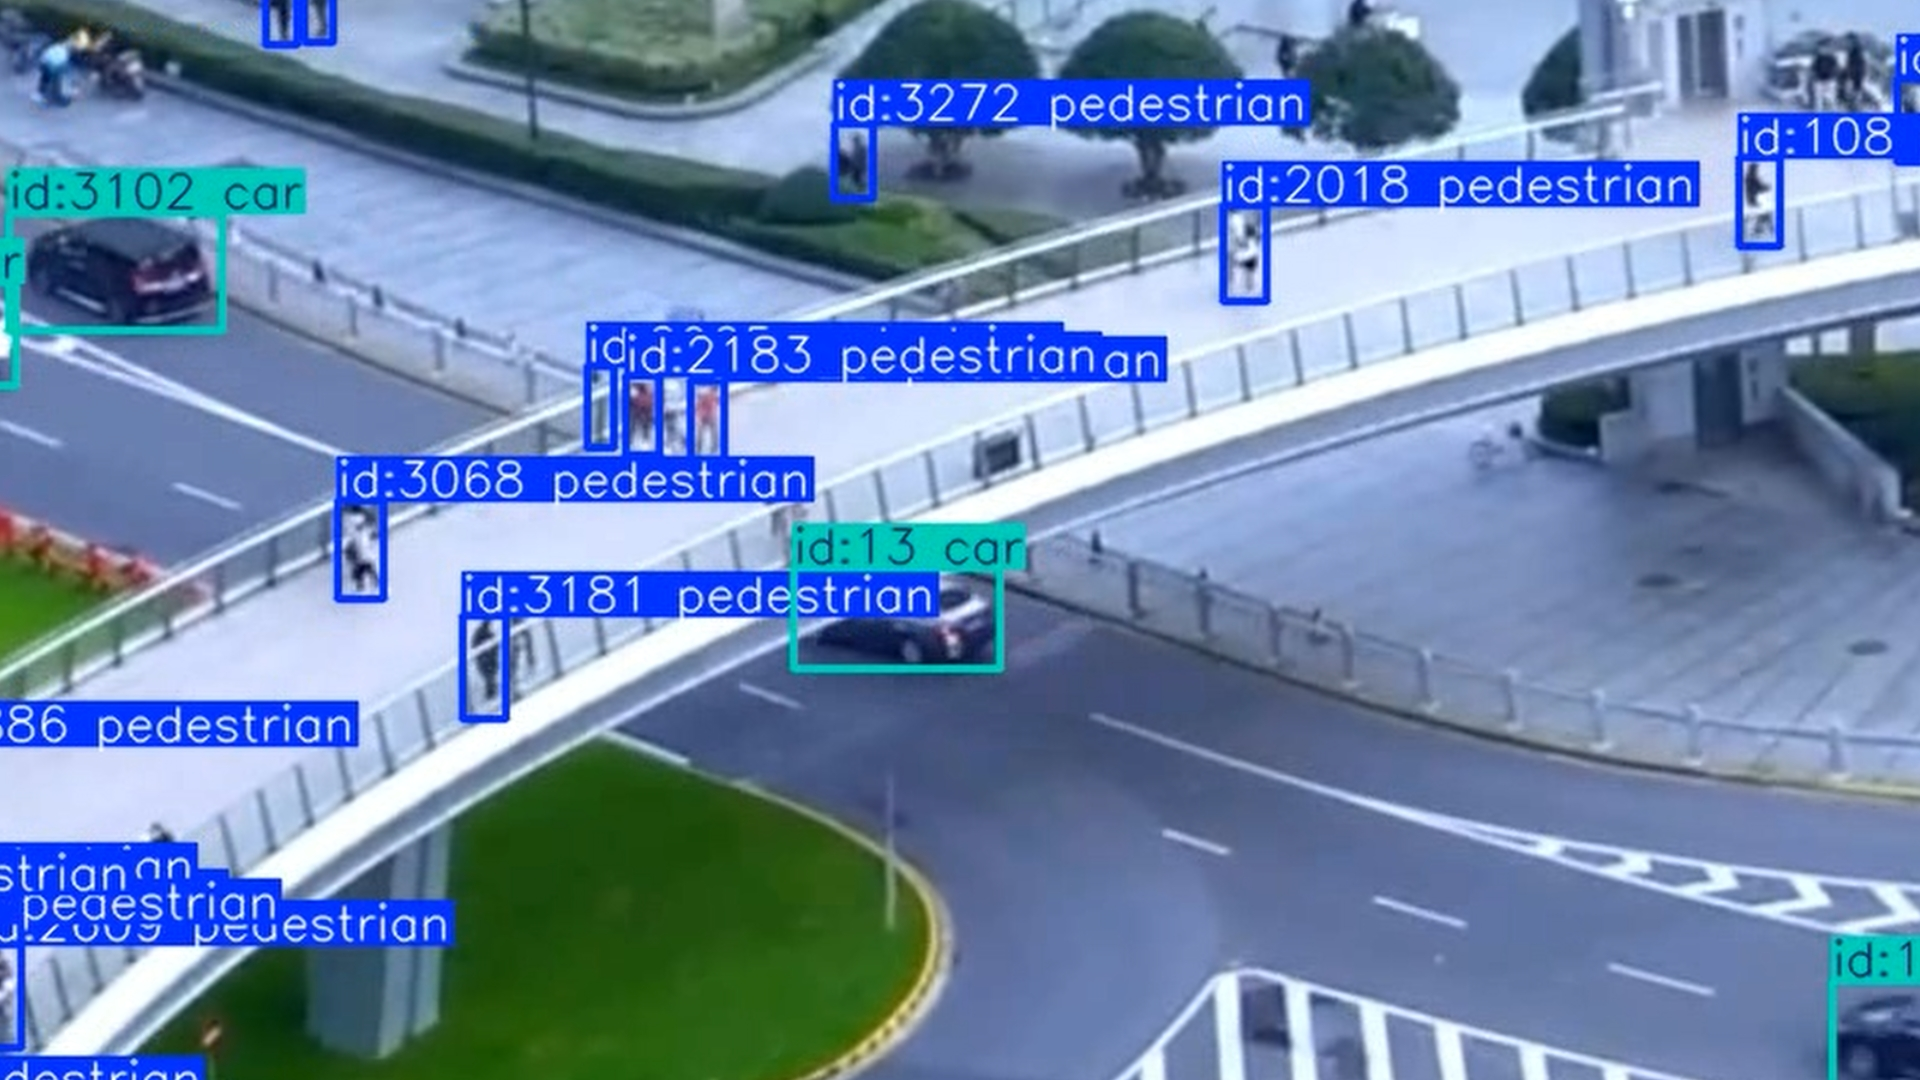
\includegraphics[width=0.24\textwidth]{figures/task2/Frames/Frame 78.jpg}
    \hfill
    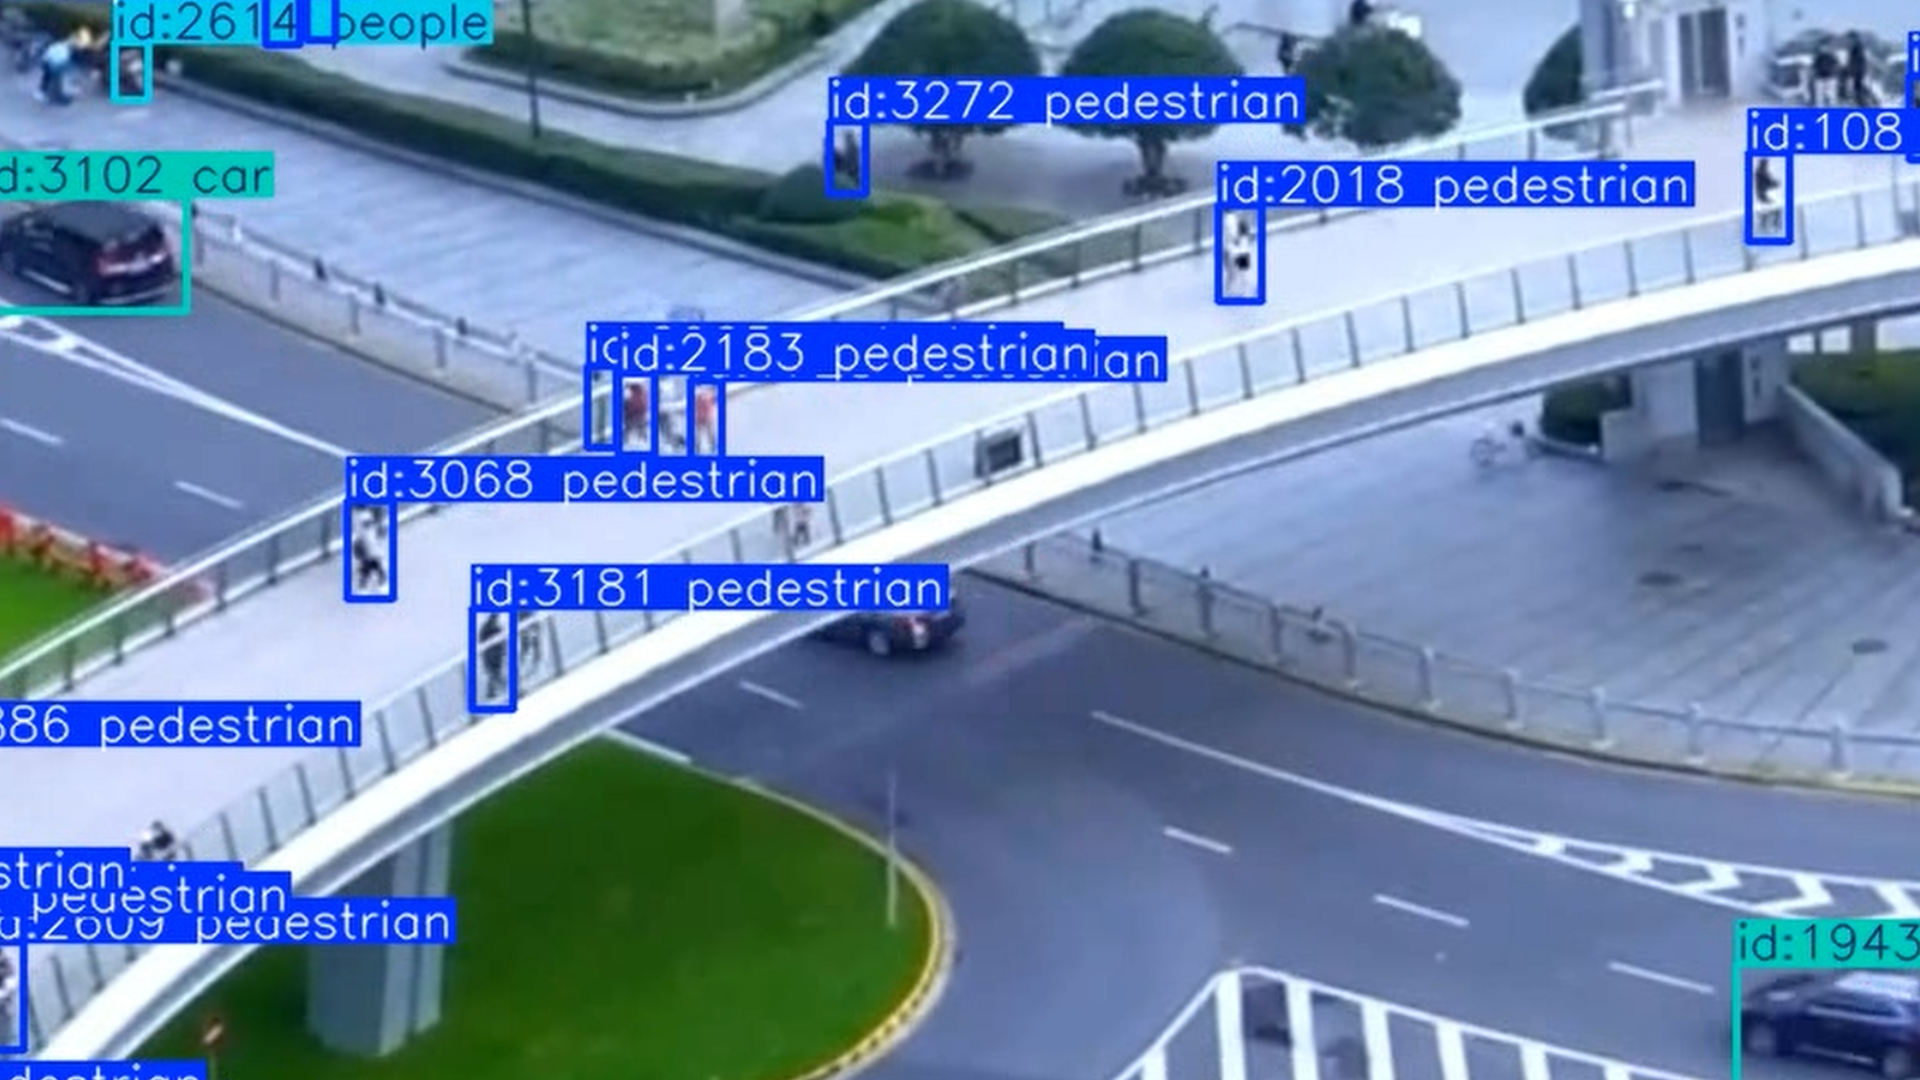
\includegraphics[width=0.24\textwidth]{figures/task2/Frames/Frame 79.jpg}
    \hfill
    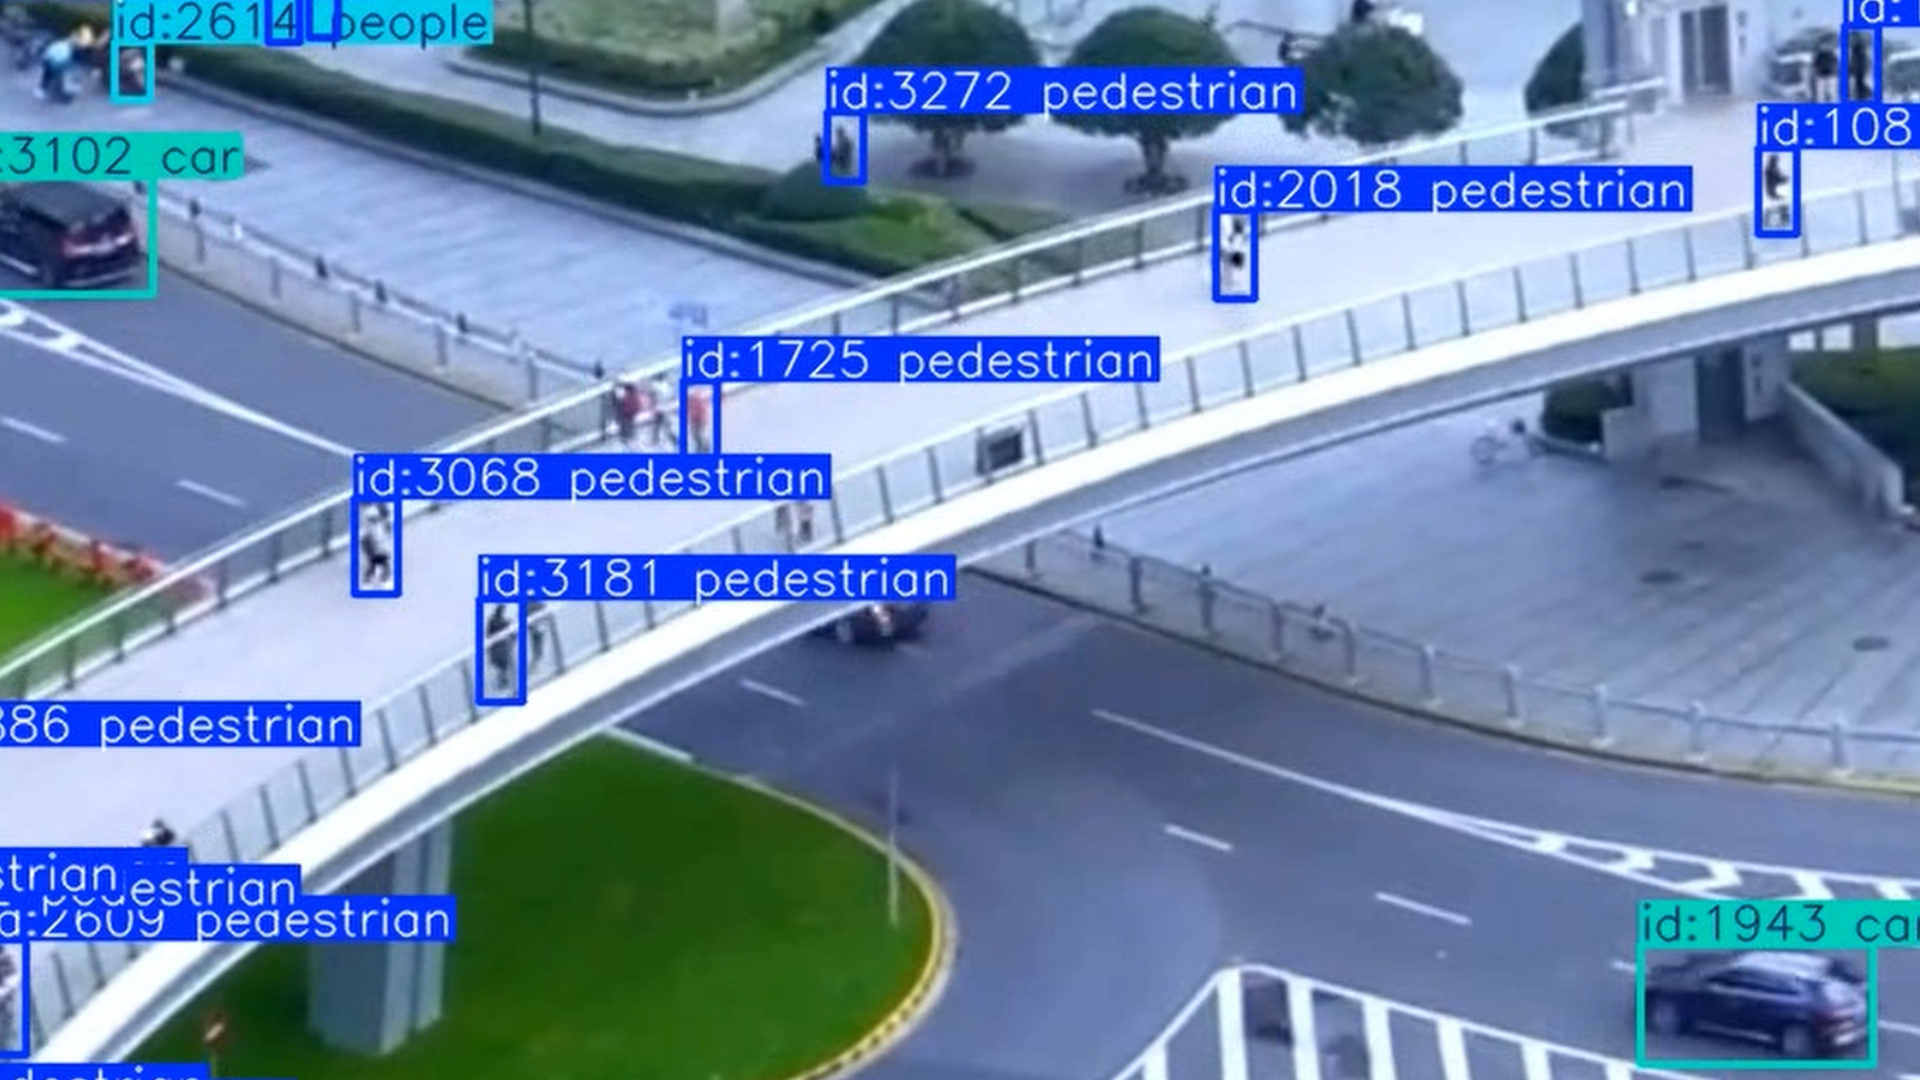
\includegraphics[width=0.24\textwidth]{figures/task2/Frames/Frame 80.jpg}
    \hfill
    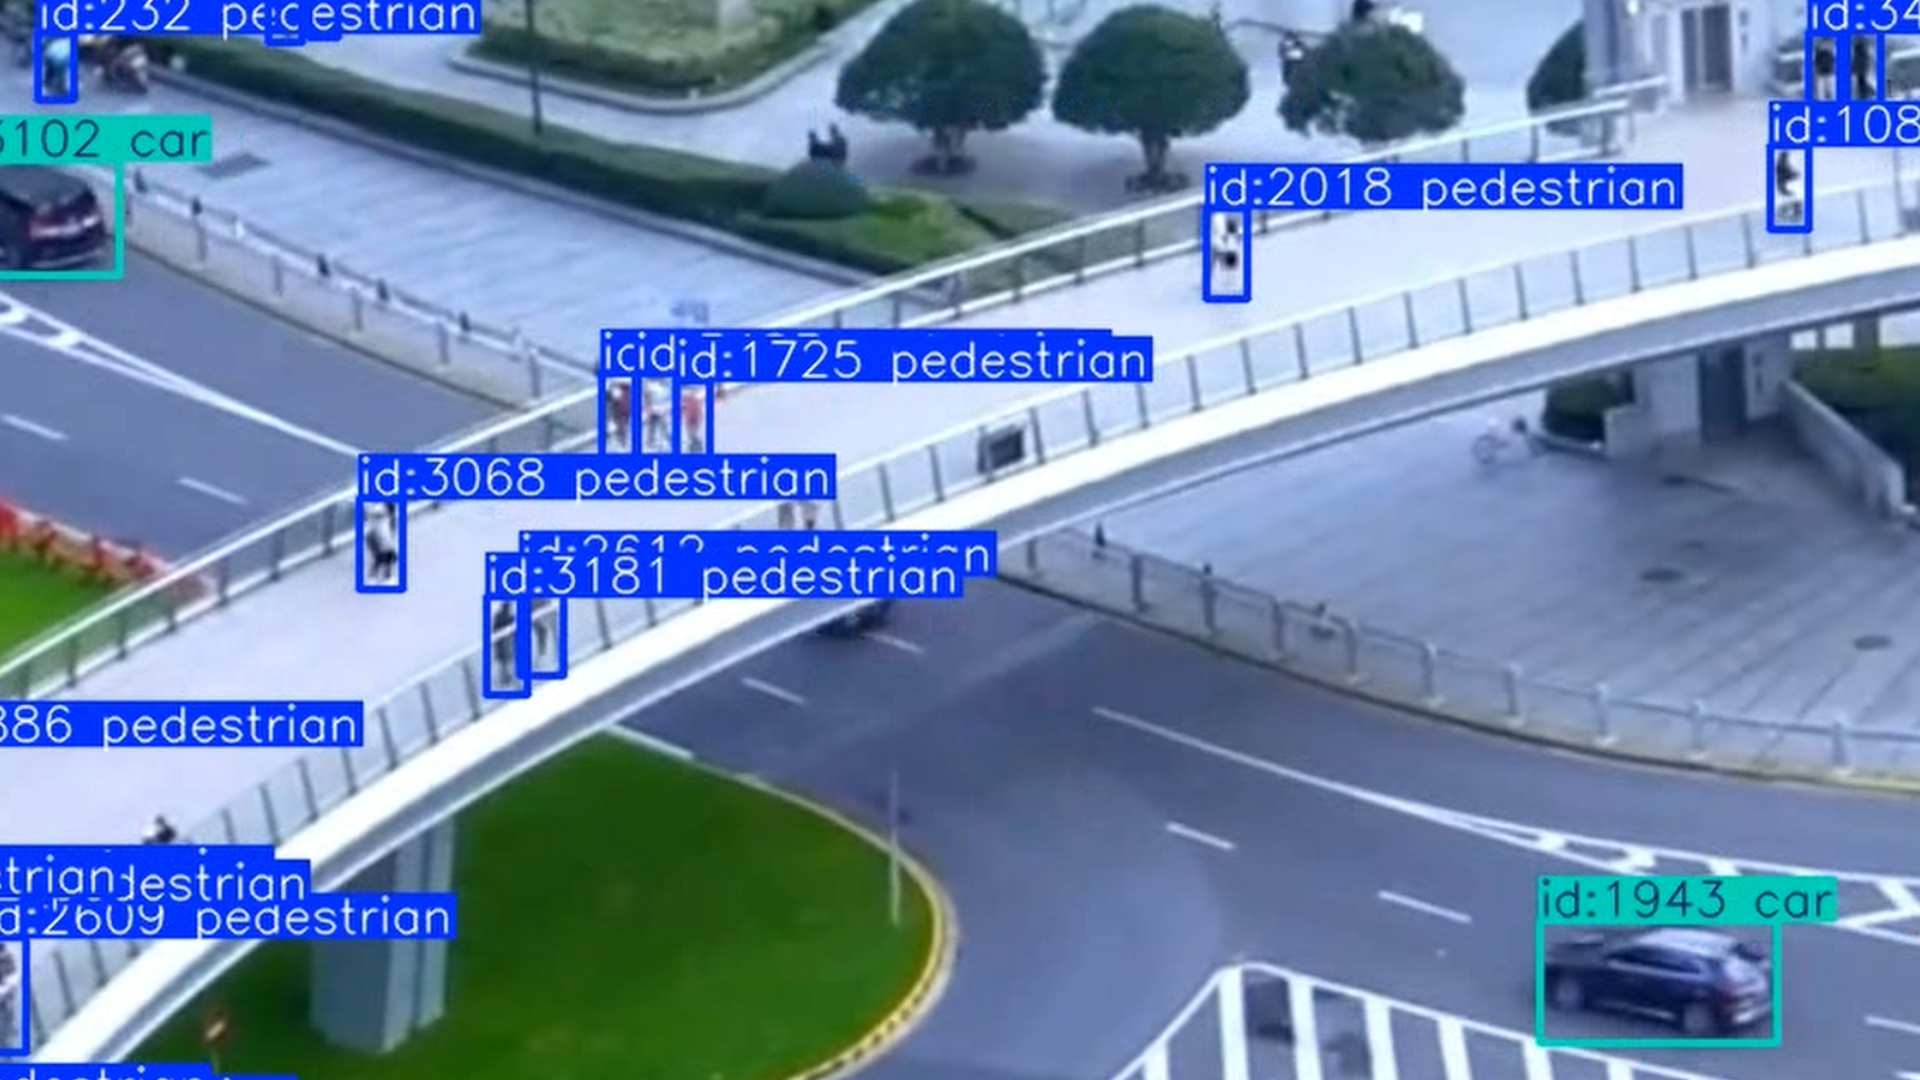
\includegraphics[width=0.24\textwidth]{figures/task2/Frames/Frame 81.jpg}

    {\hspace{0.07\linewidth}\small Frame 78 \hfill Frame 79 \hfill Frame 80 \hfill Frame 81\hspace{0.07\linewidth}}

    \vspace{0.3em}

    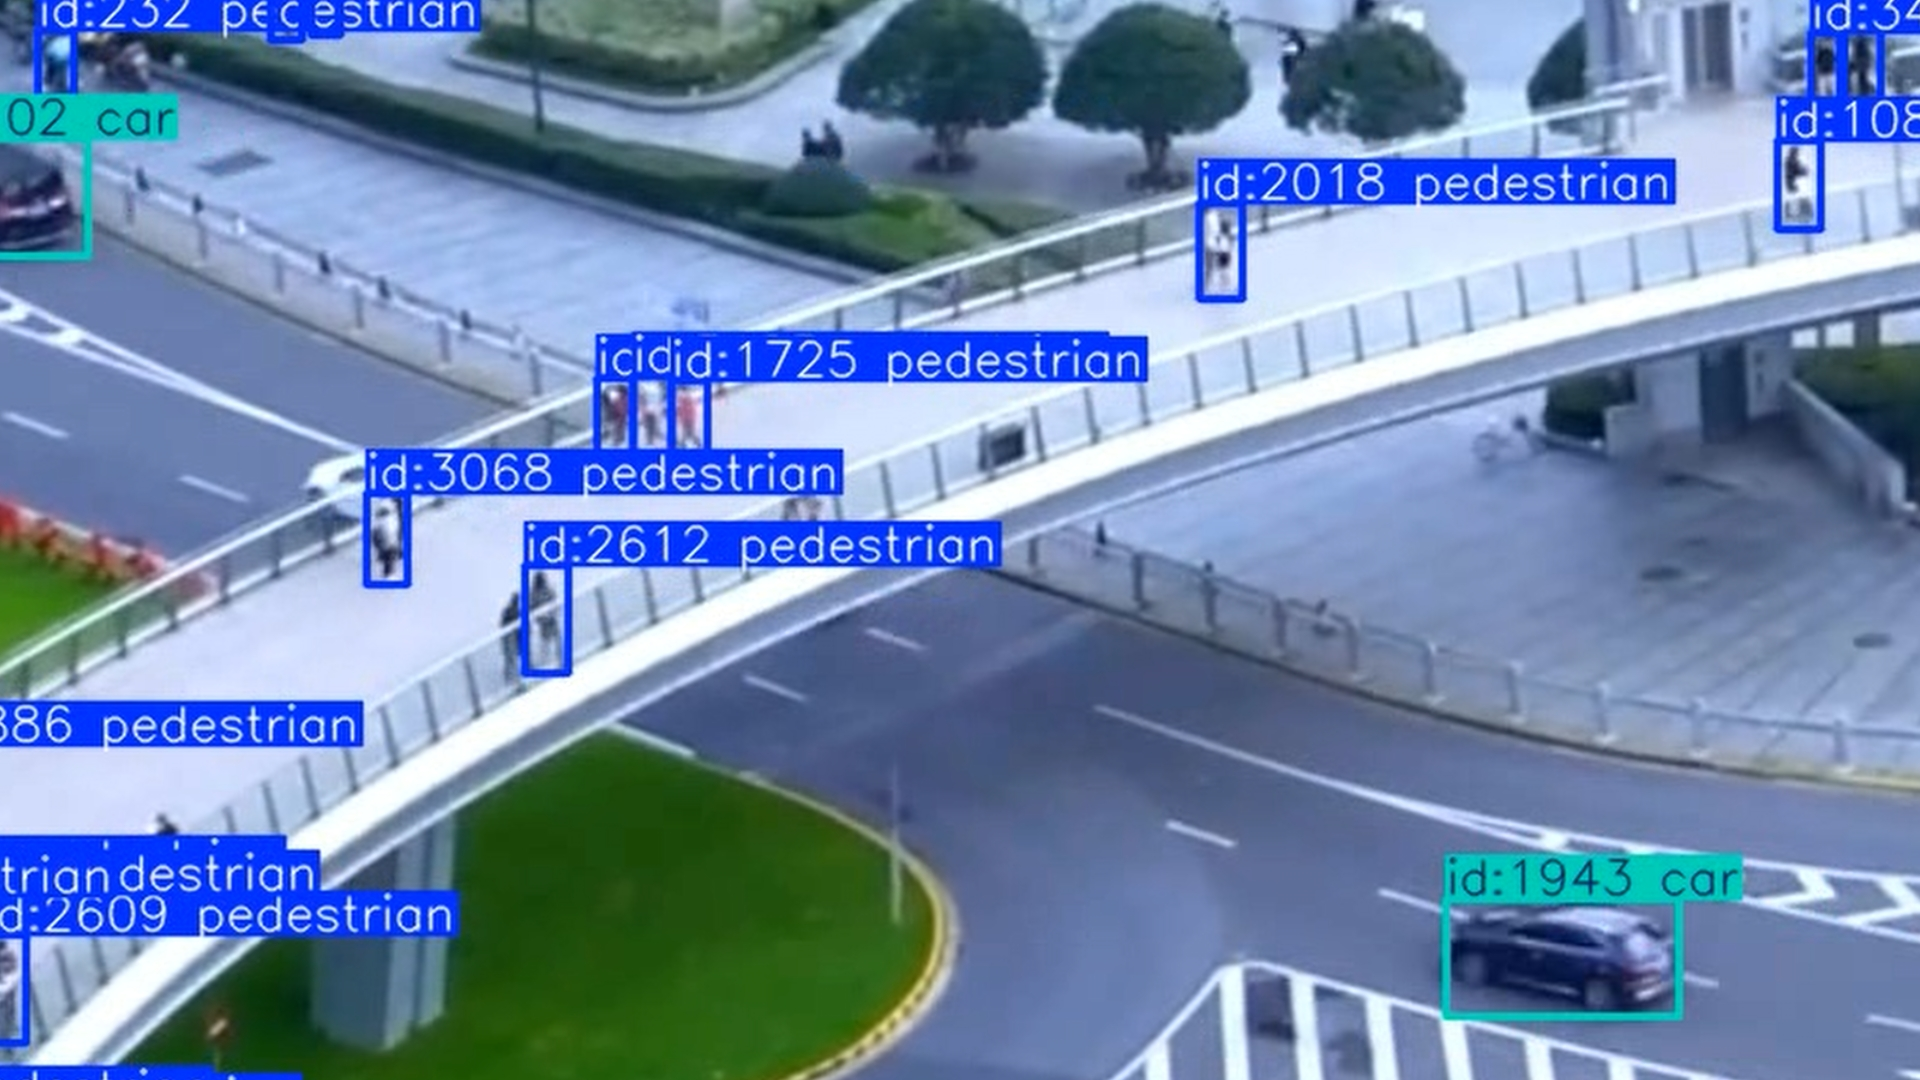
\includegraphics[width=0.24\textwidth]{figures/task2/Frames/Frame 82.jpg}
    \hfill
    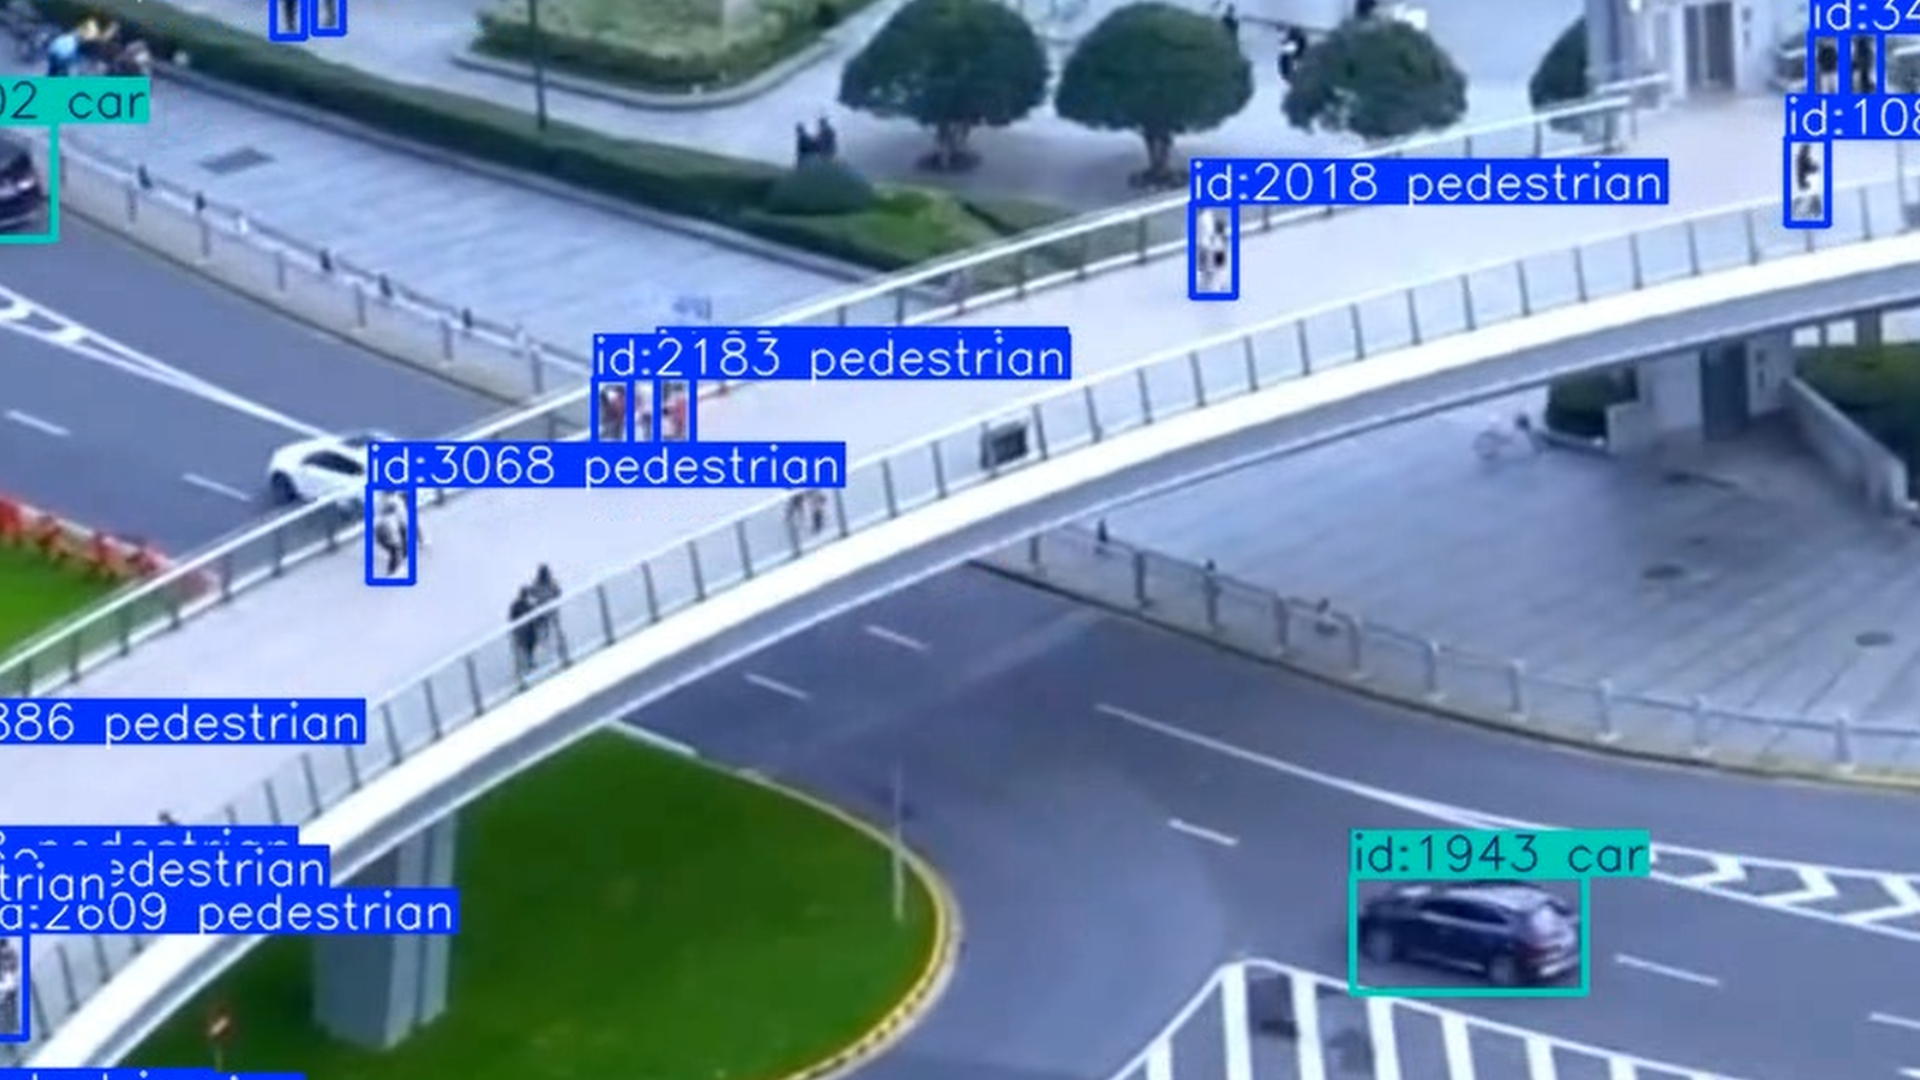
\includegraphics[width=0.24\textwidth]{figures/task2/Frames/Frame 83.jpg}
    \hfill
    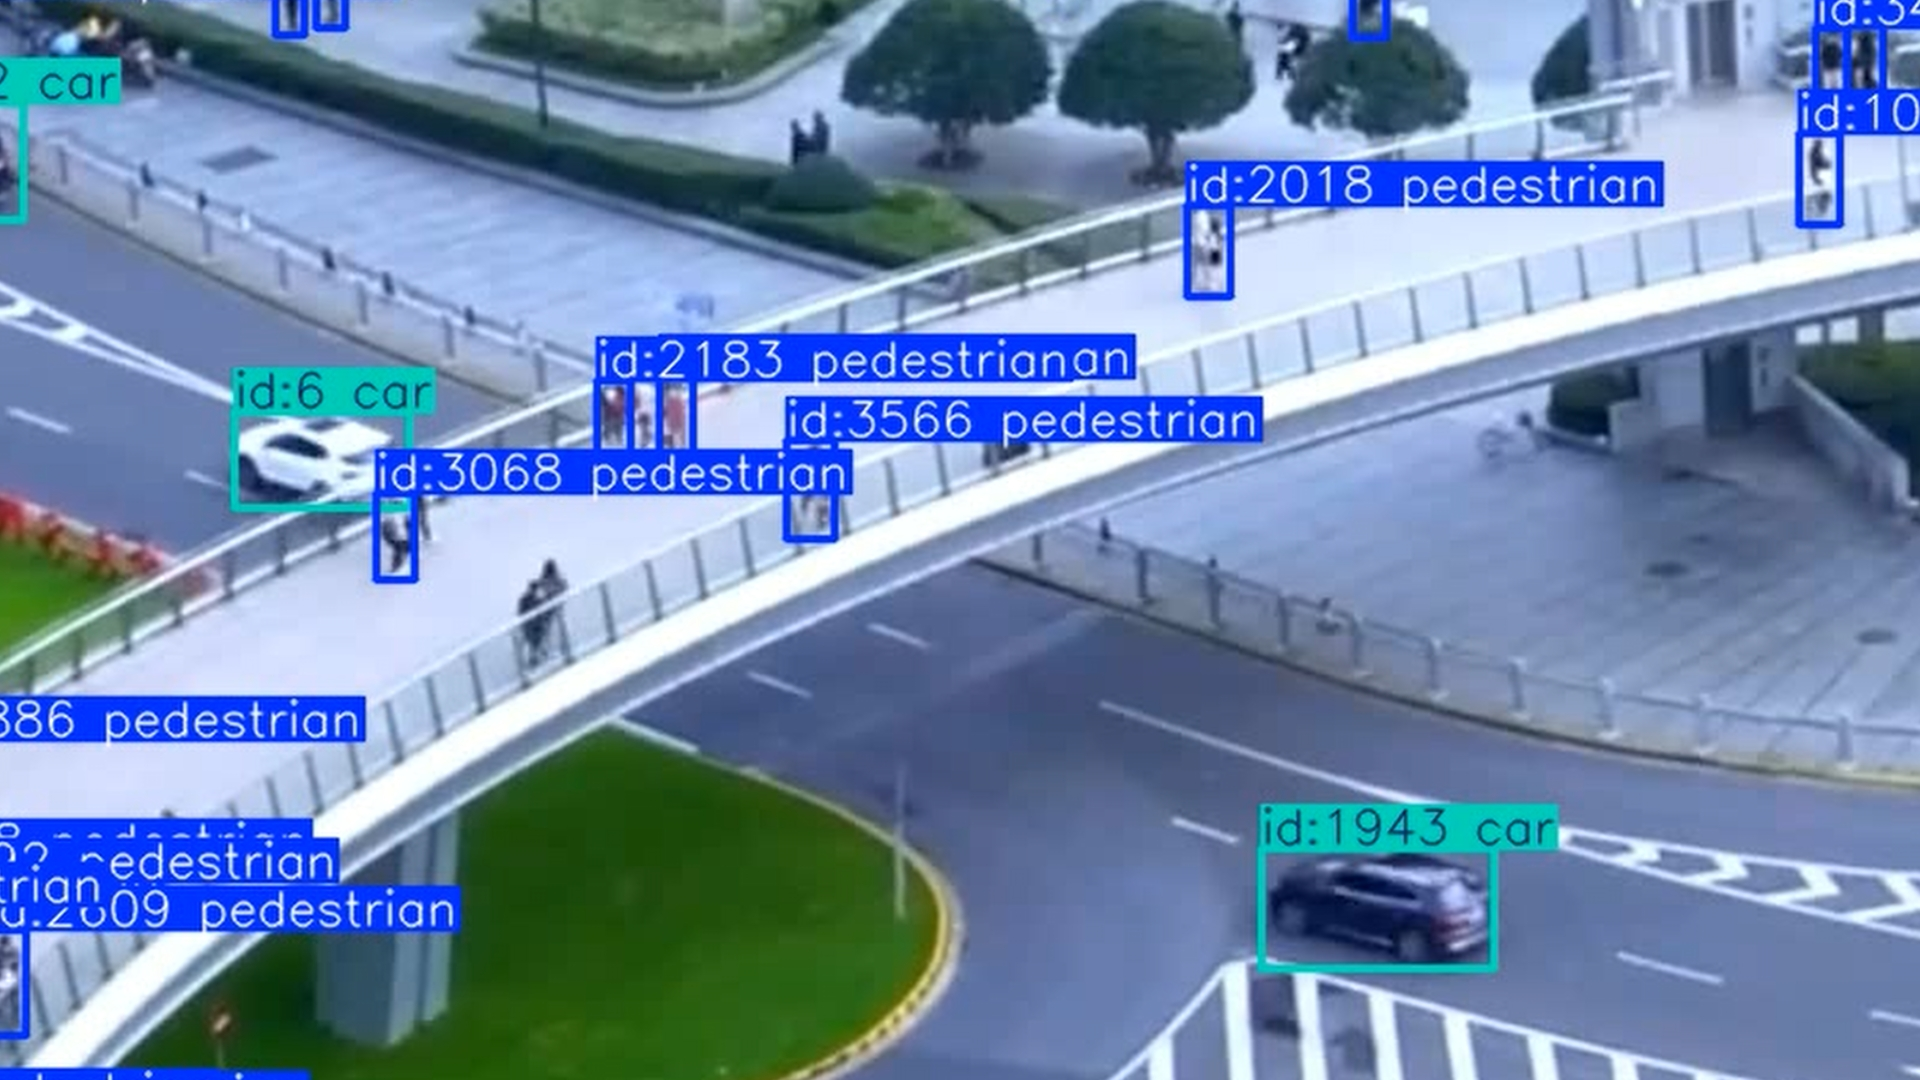
\includegraphics[width=0.24\textwidth]{figures/task2/Frames/Frame 84.jpg}
    \hfill
    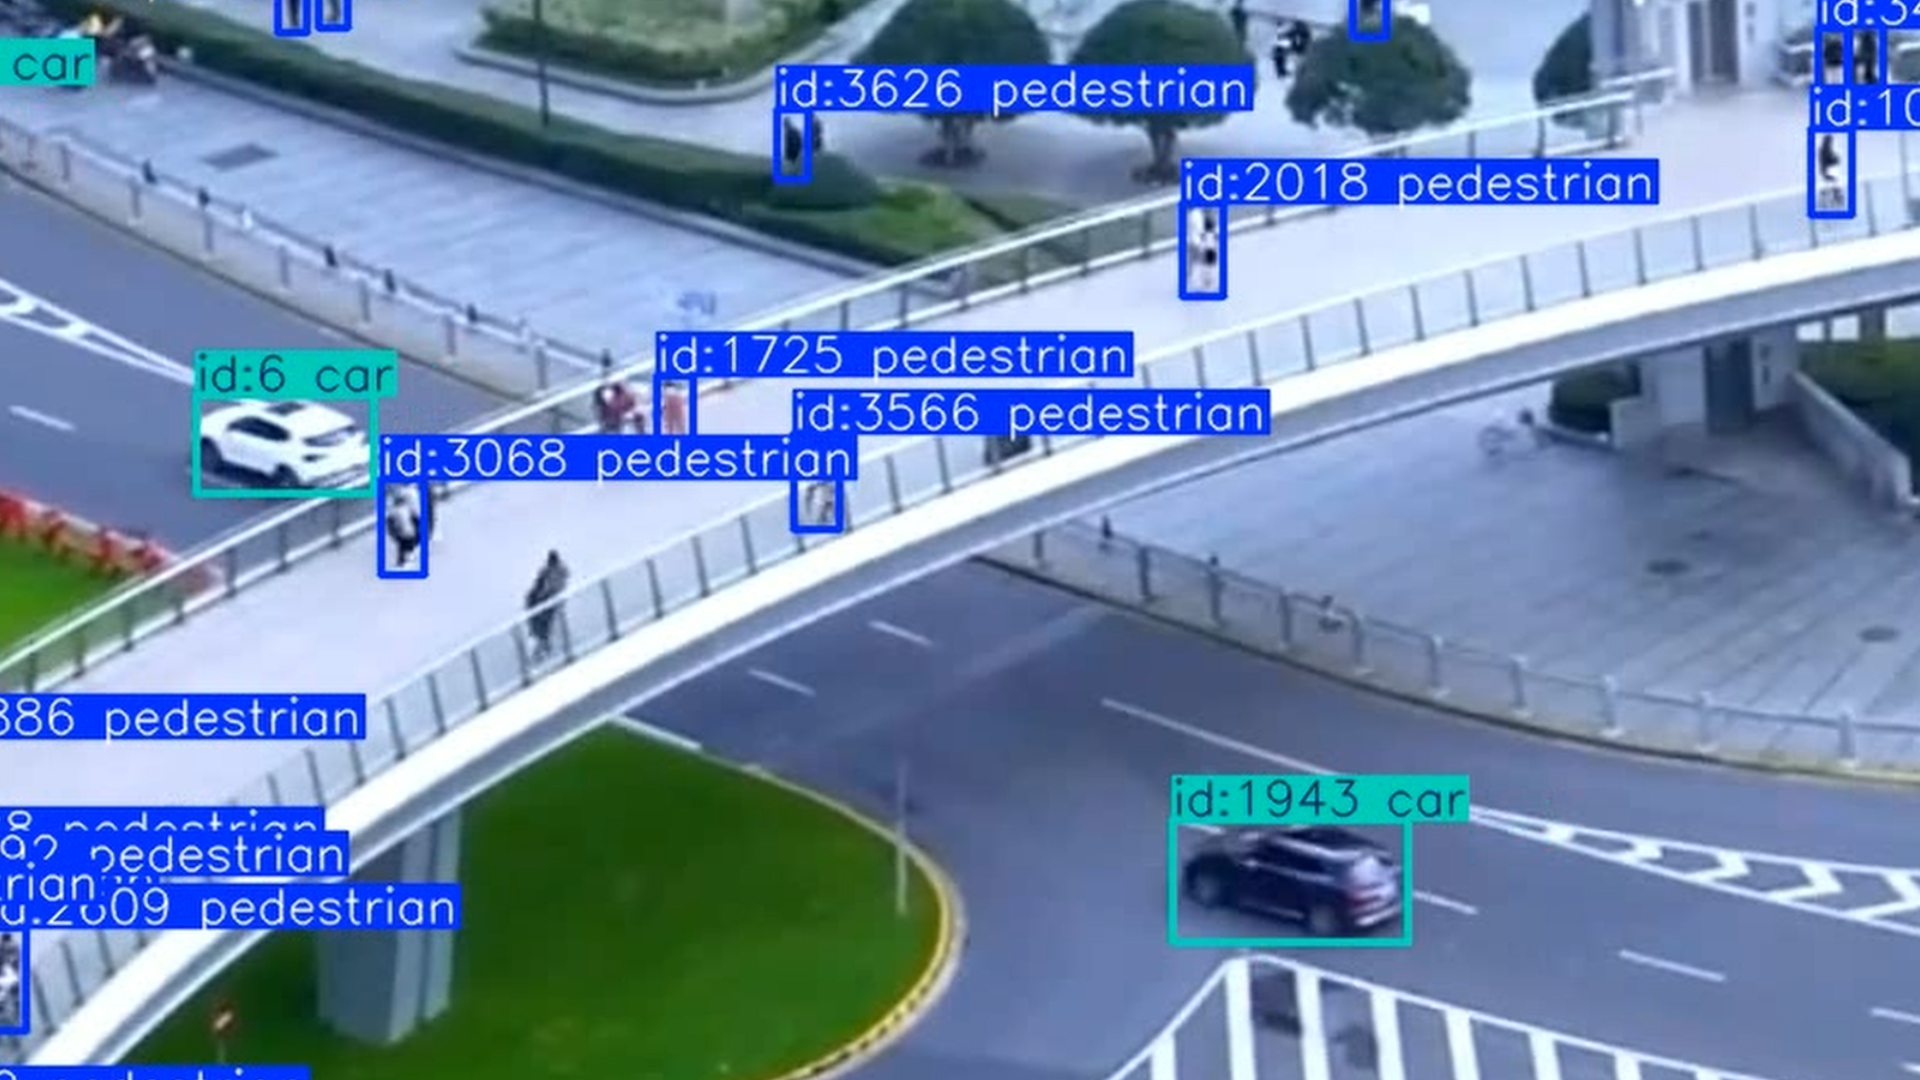
\includegraphics[width=0.24\textwidth]{figures/task2/Frames/Frame 85.jpg}

    {\hspace{0.07\linewidth}\small Frame 82 \hfill Frame 83 \hfill Frame 84 \hfill Frame 85\hspace{0.07\linewidth}}

    \vspace{0.3em}

    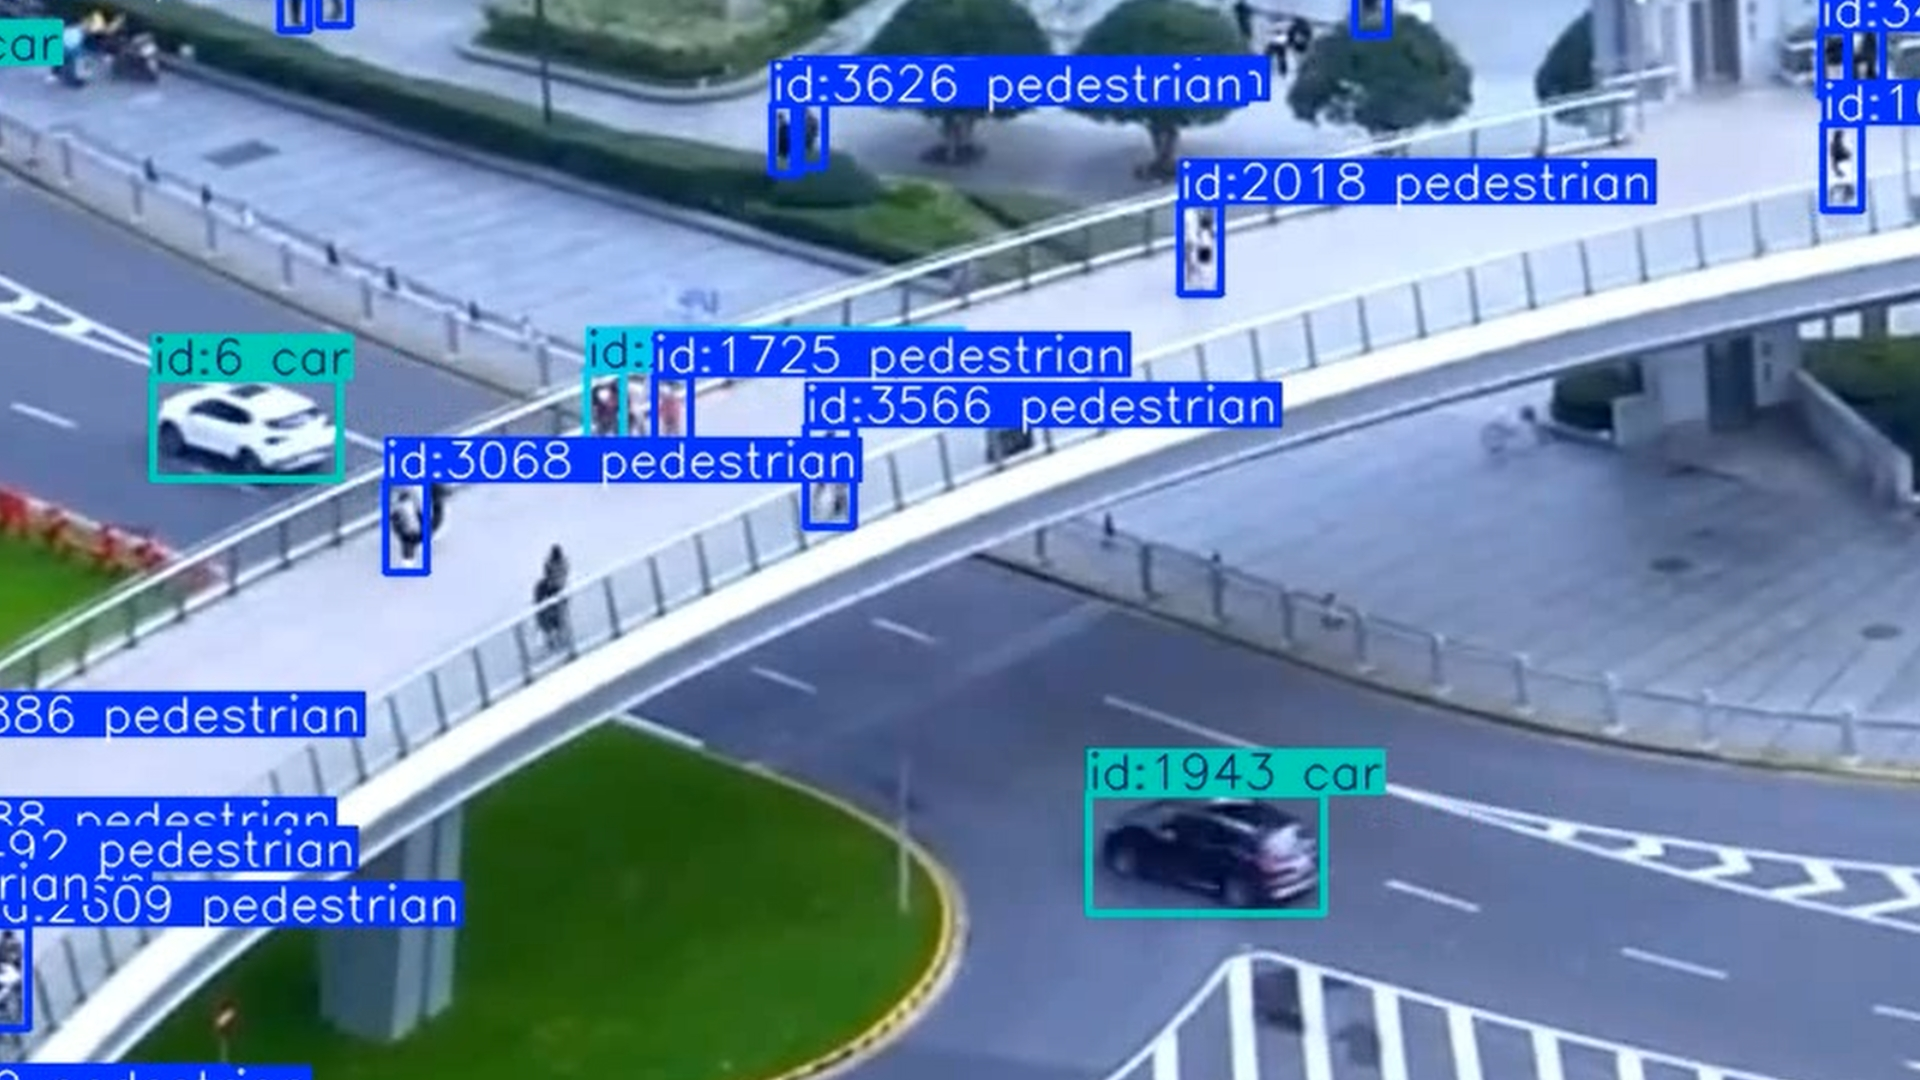
\includegraphics[width=0.24\textwidth]{figures/task2/Frames/Frame 86.jpg}
    \hfill
    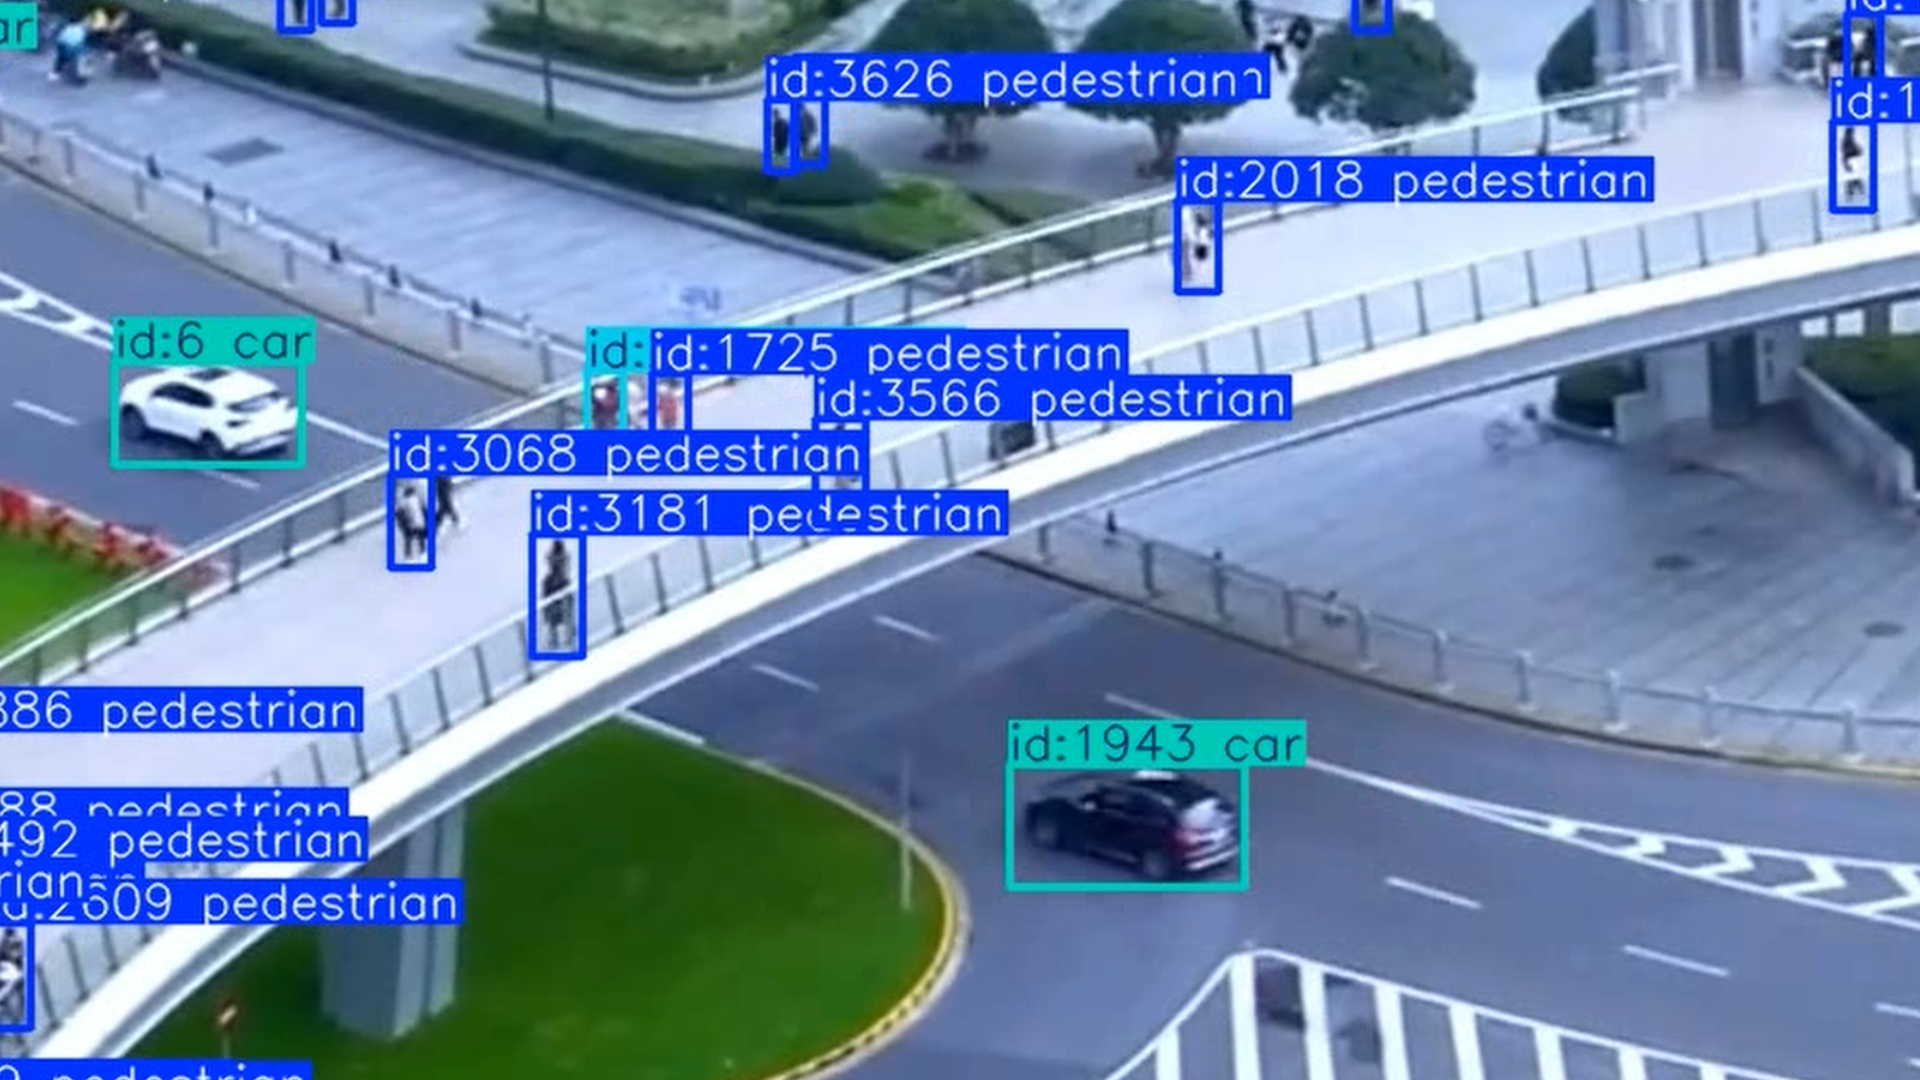
\includegraphics[width=0.24\textwidth]{figures/task2/Frames/Frame 87.jpg}
    \hfill
    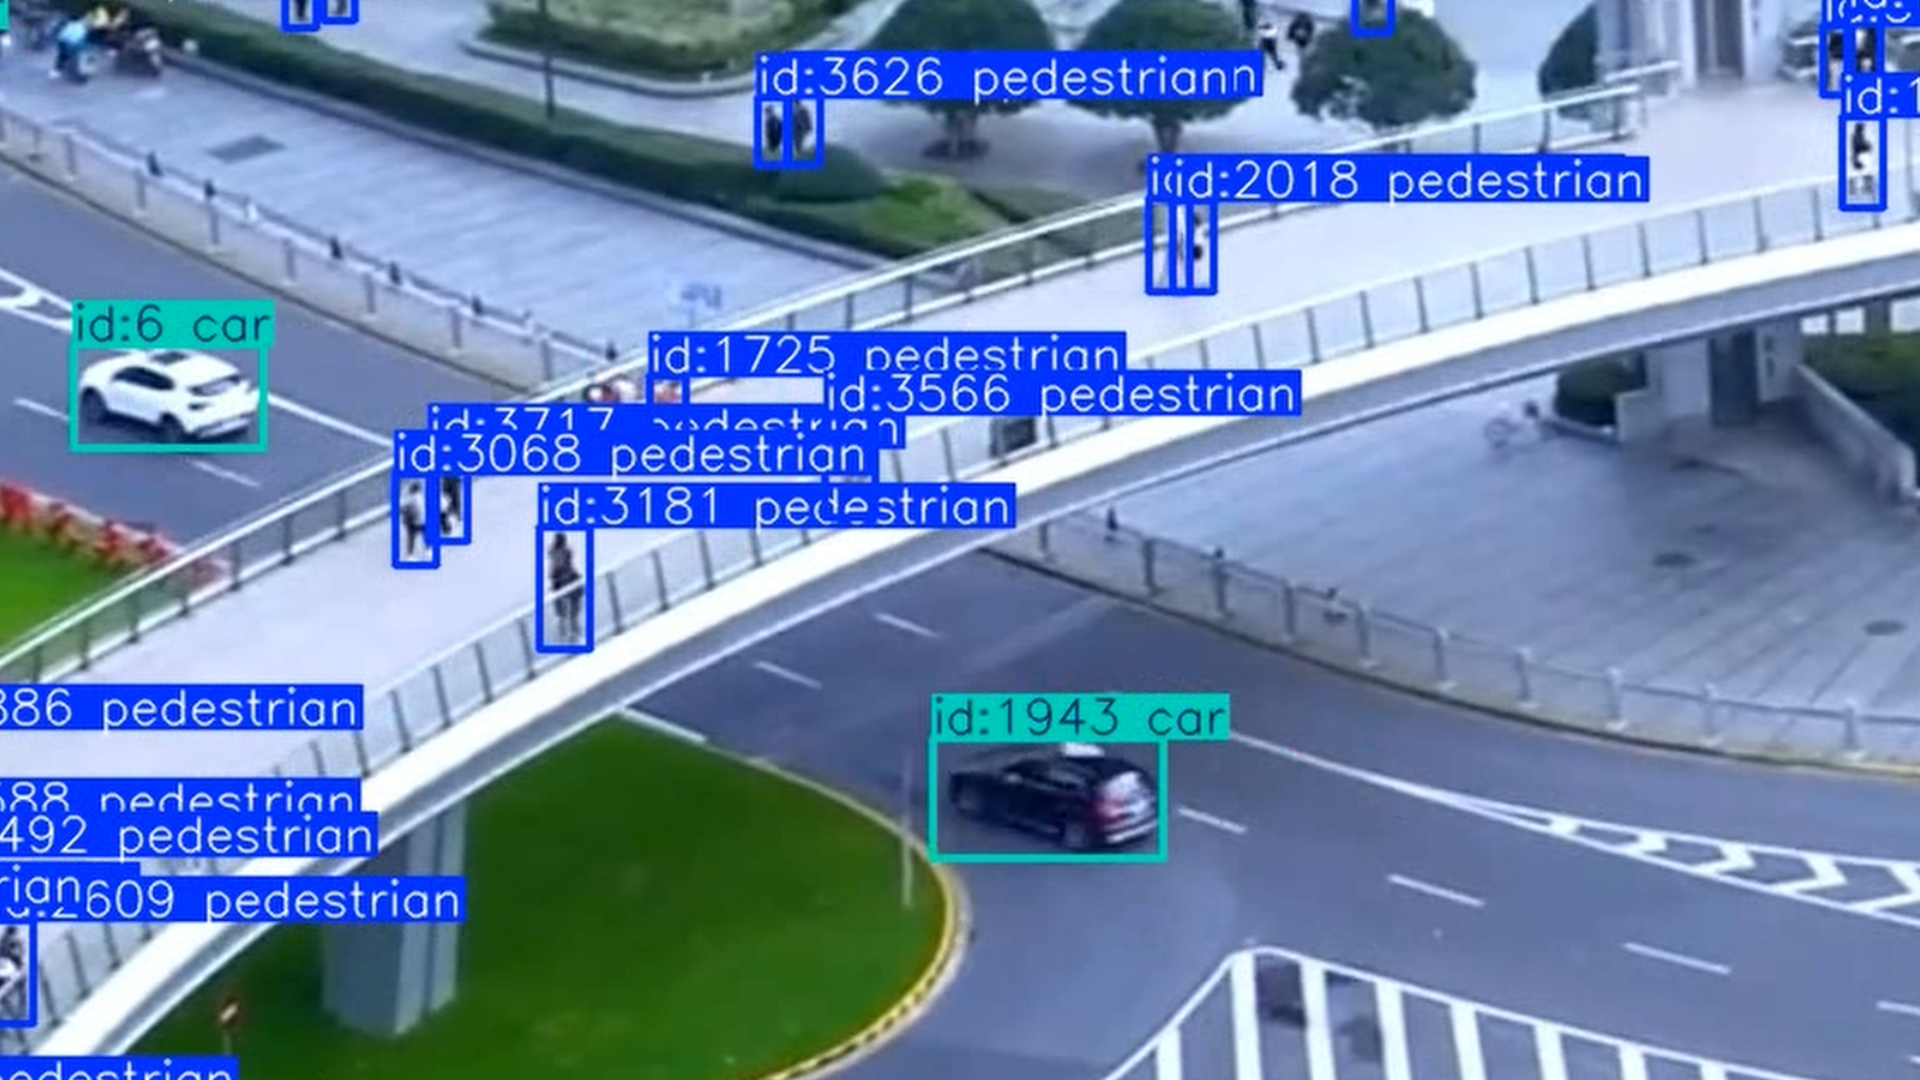
\includegraphics[width=0.24\textwidth]{figures/task2/Frames/Frame 88.jpg}
    \hfill
    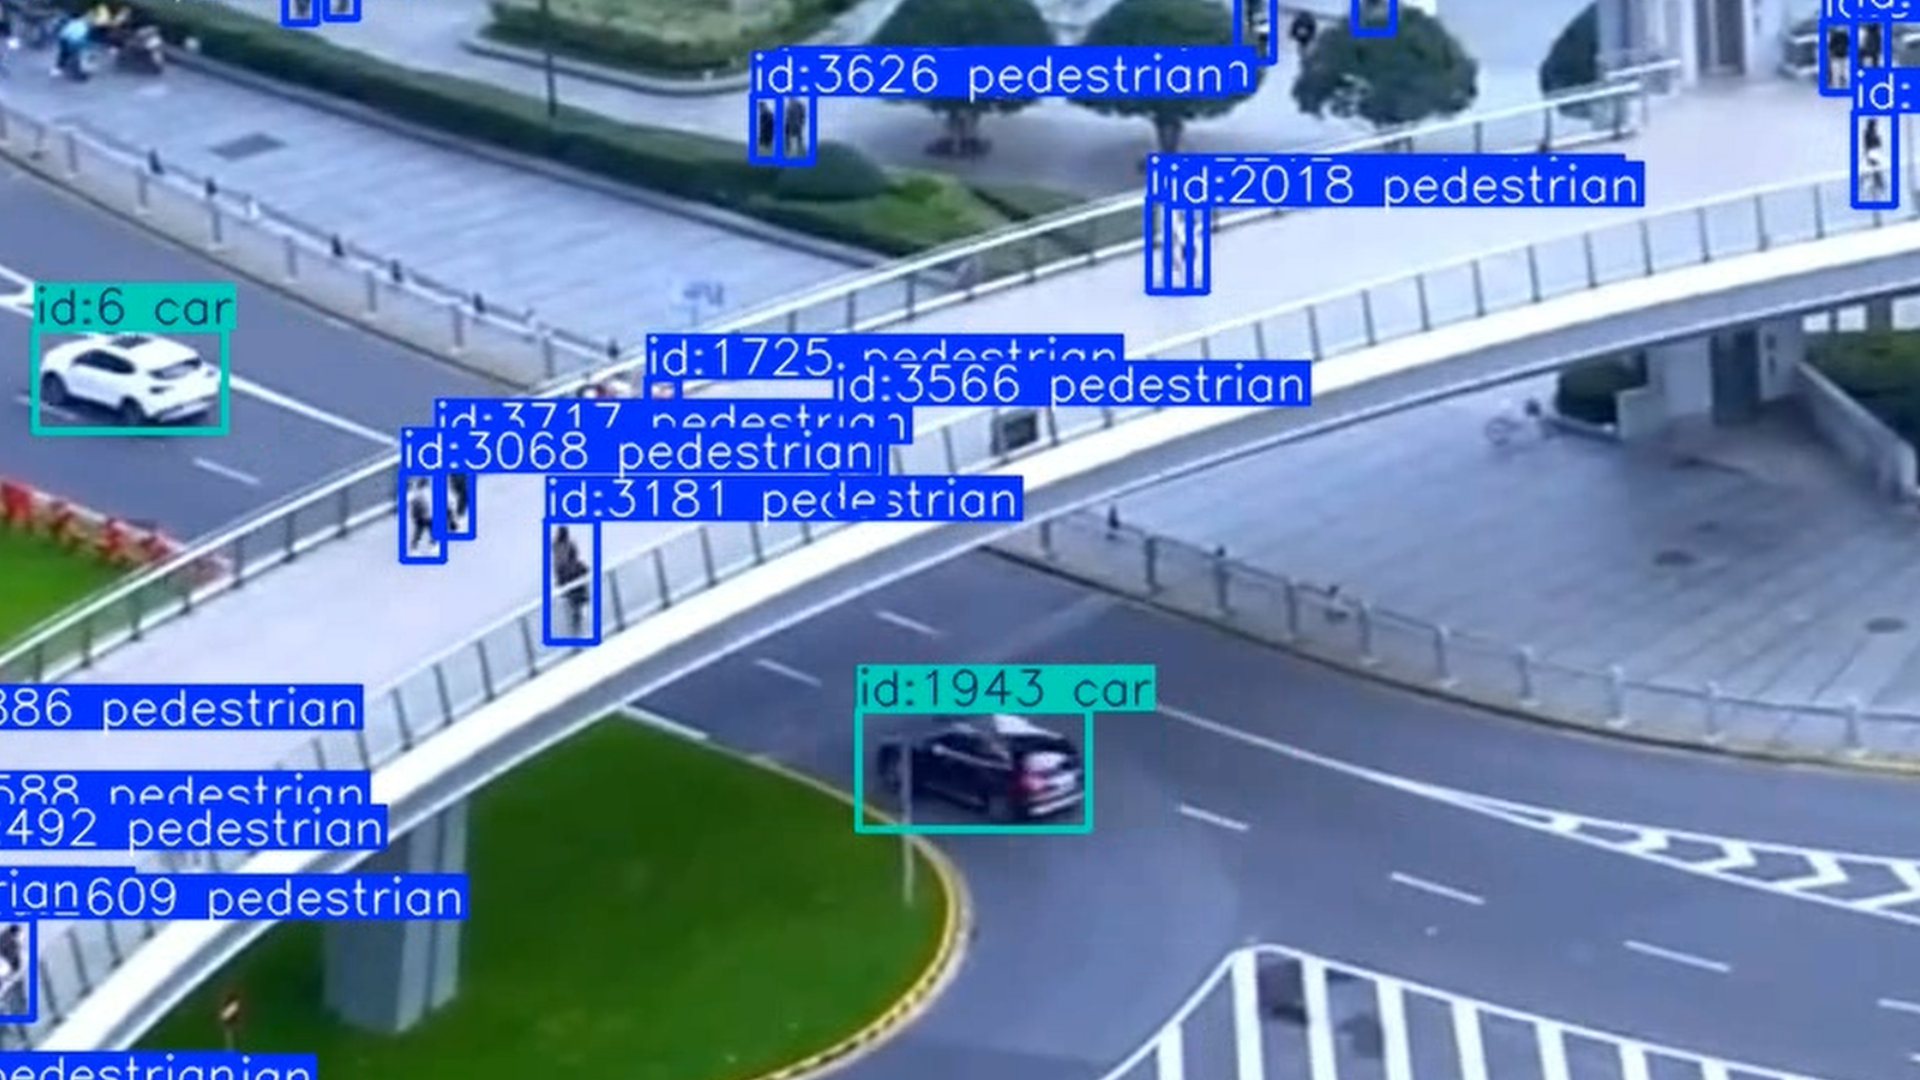
\includegraphics[width=0.24\textwidth]{figures/task2/Frames/Frame 89.jpg}

    {\hspace{0.07\linewidth}\small Frame 86 \hfill Frame 87 \hfill Frame 88 \hfill Frame 89\hspace{0.07\linewidth}}

    \vspace{0.3em}

    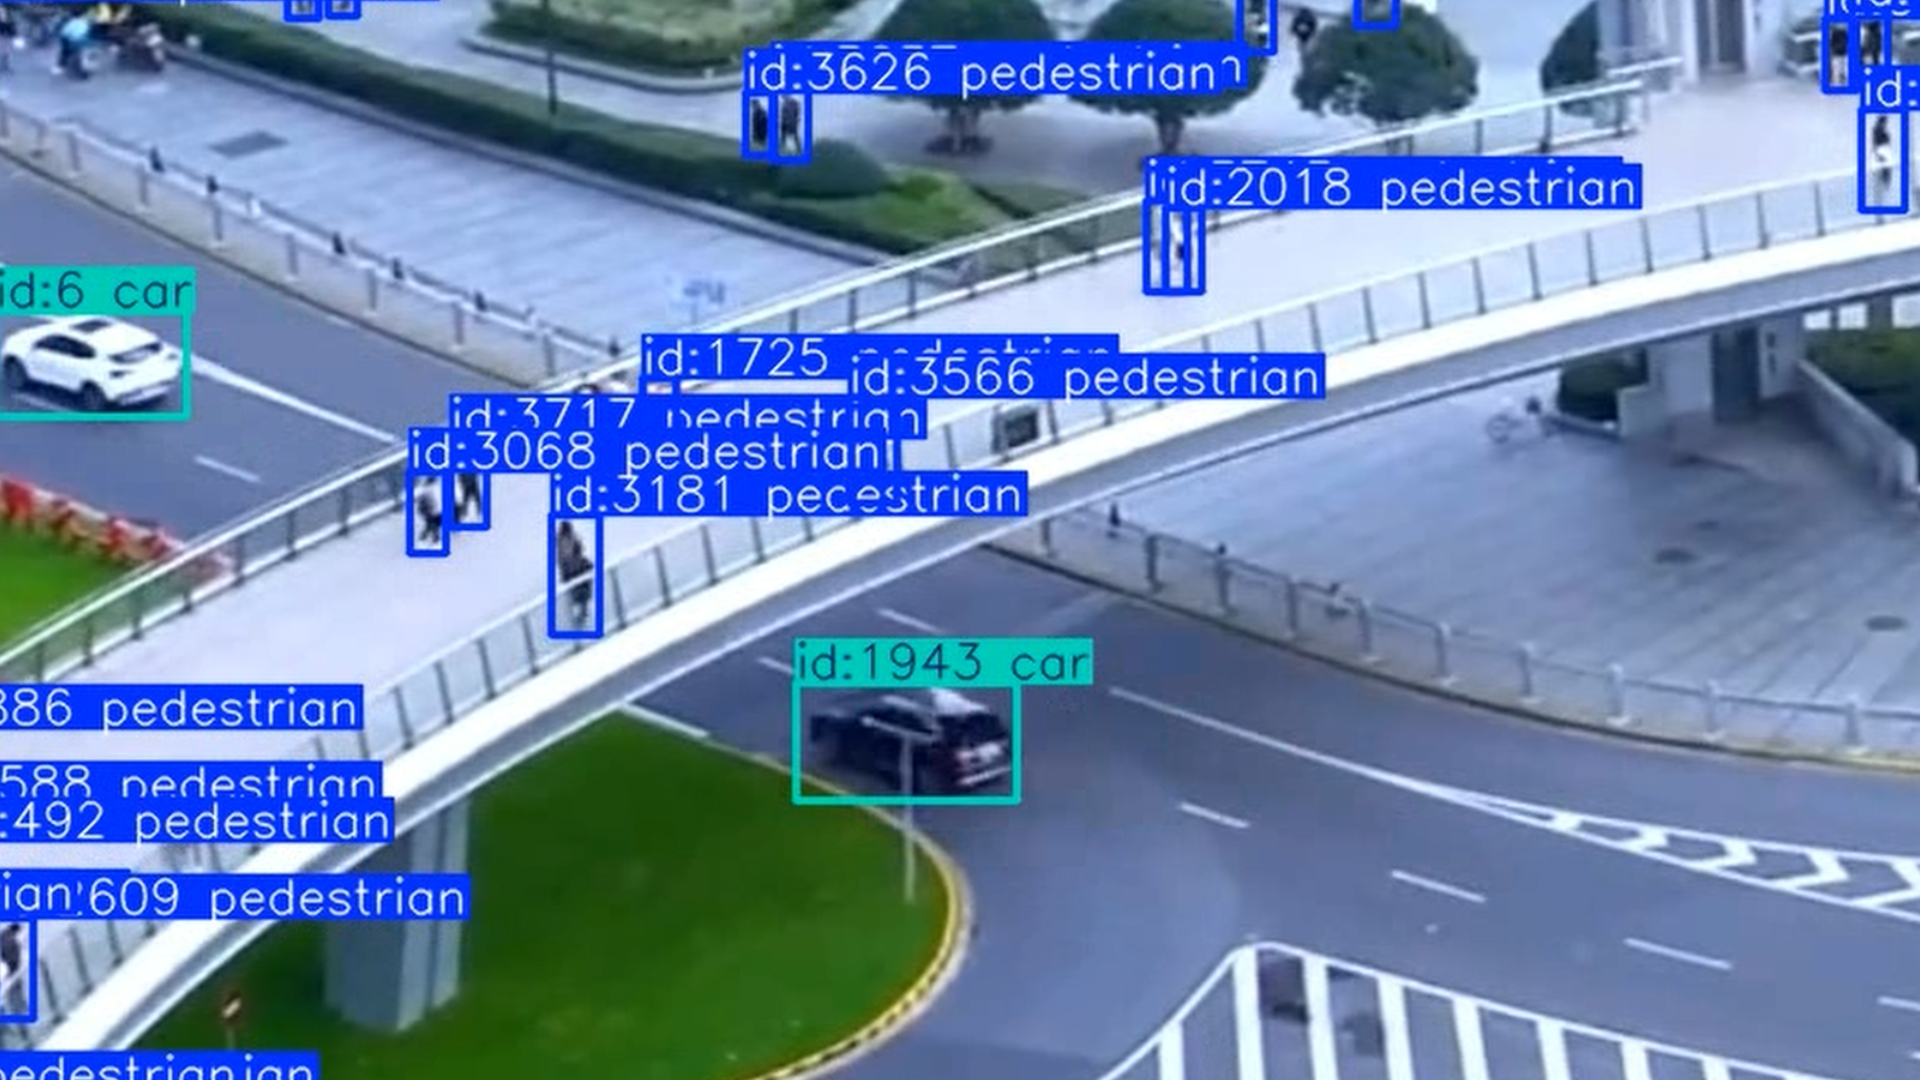
\includegraphics[width=0.24\textwidth]{figures/task2/Frames/Frame 90.jpg}
    \hfill
    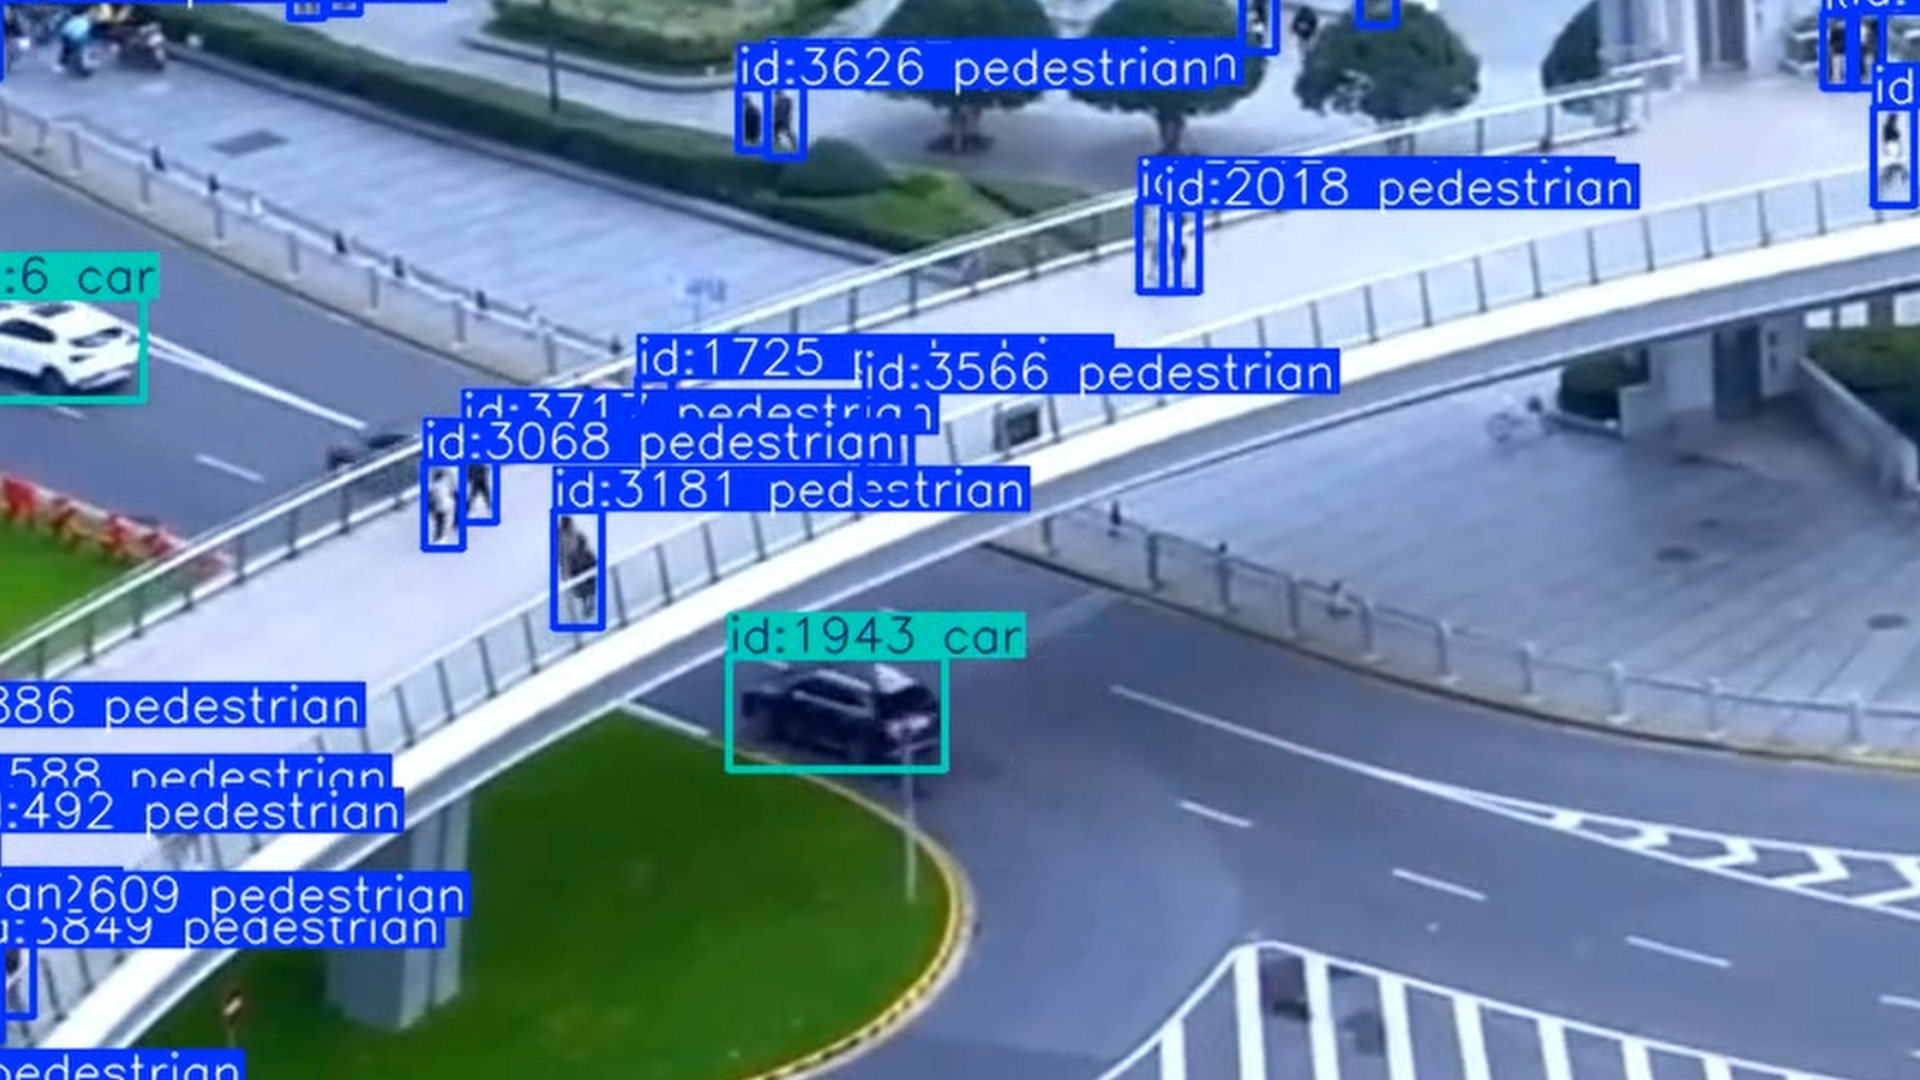
\includegraphics[width=0.24\textwidth]{figures/task2/Frames/Frame 91.jpg}
    \hfill
    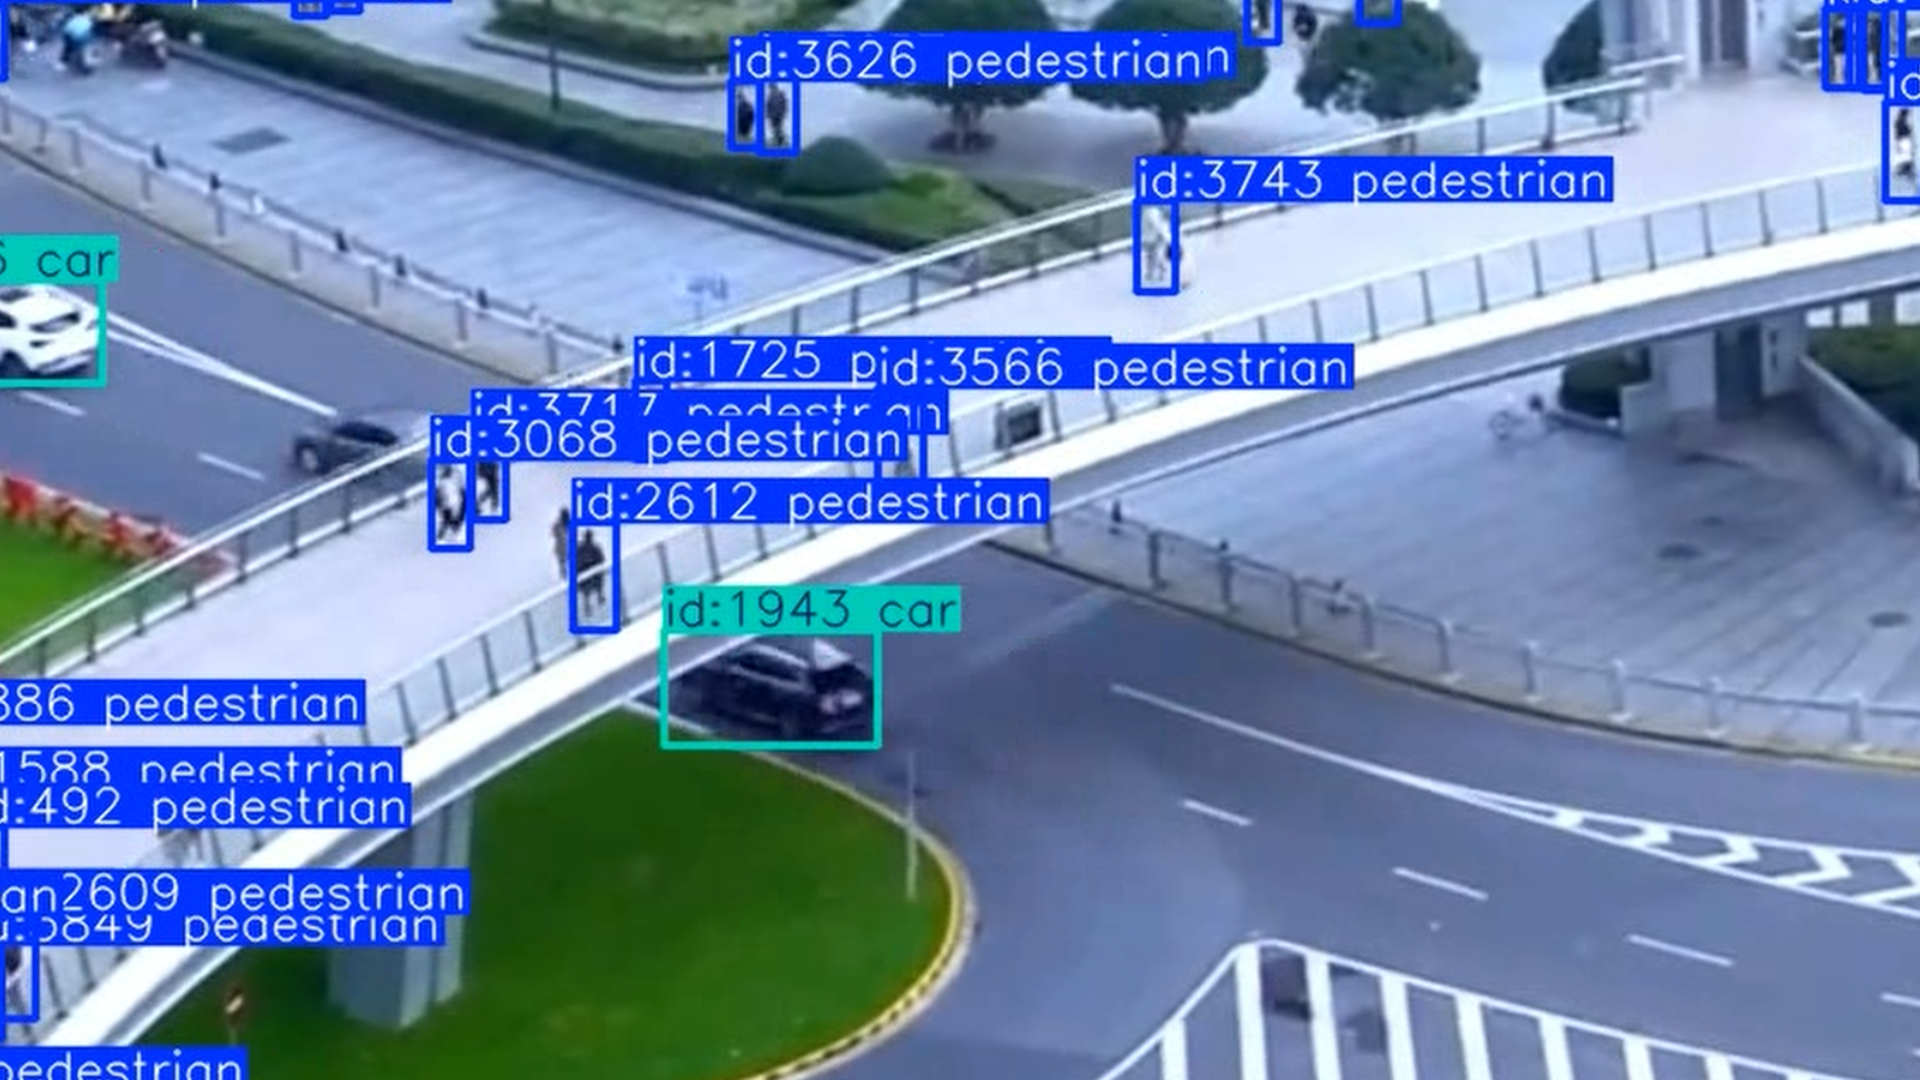
\includegraphics[width=0.24\textwidth]{figures/task2/Frames/Frame 92.jpg}
    \hfill
    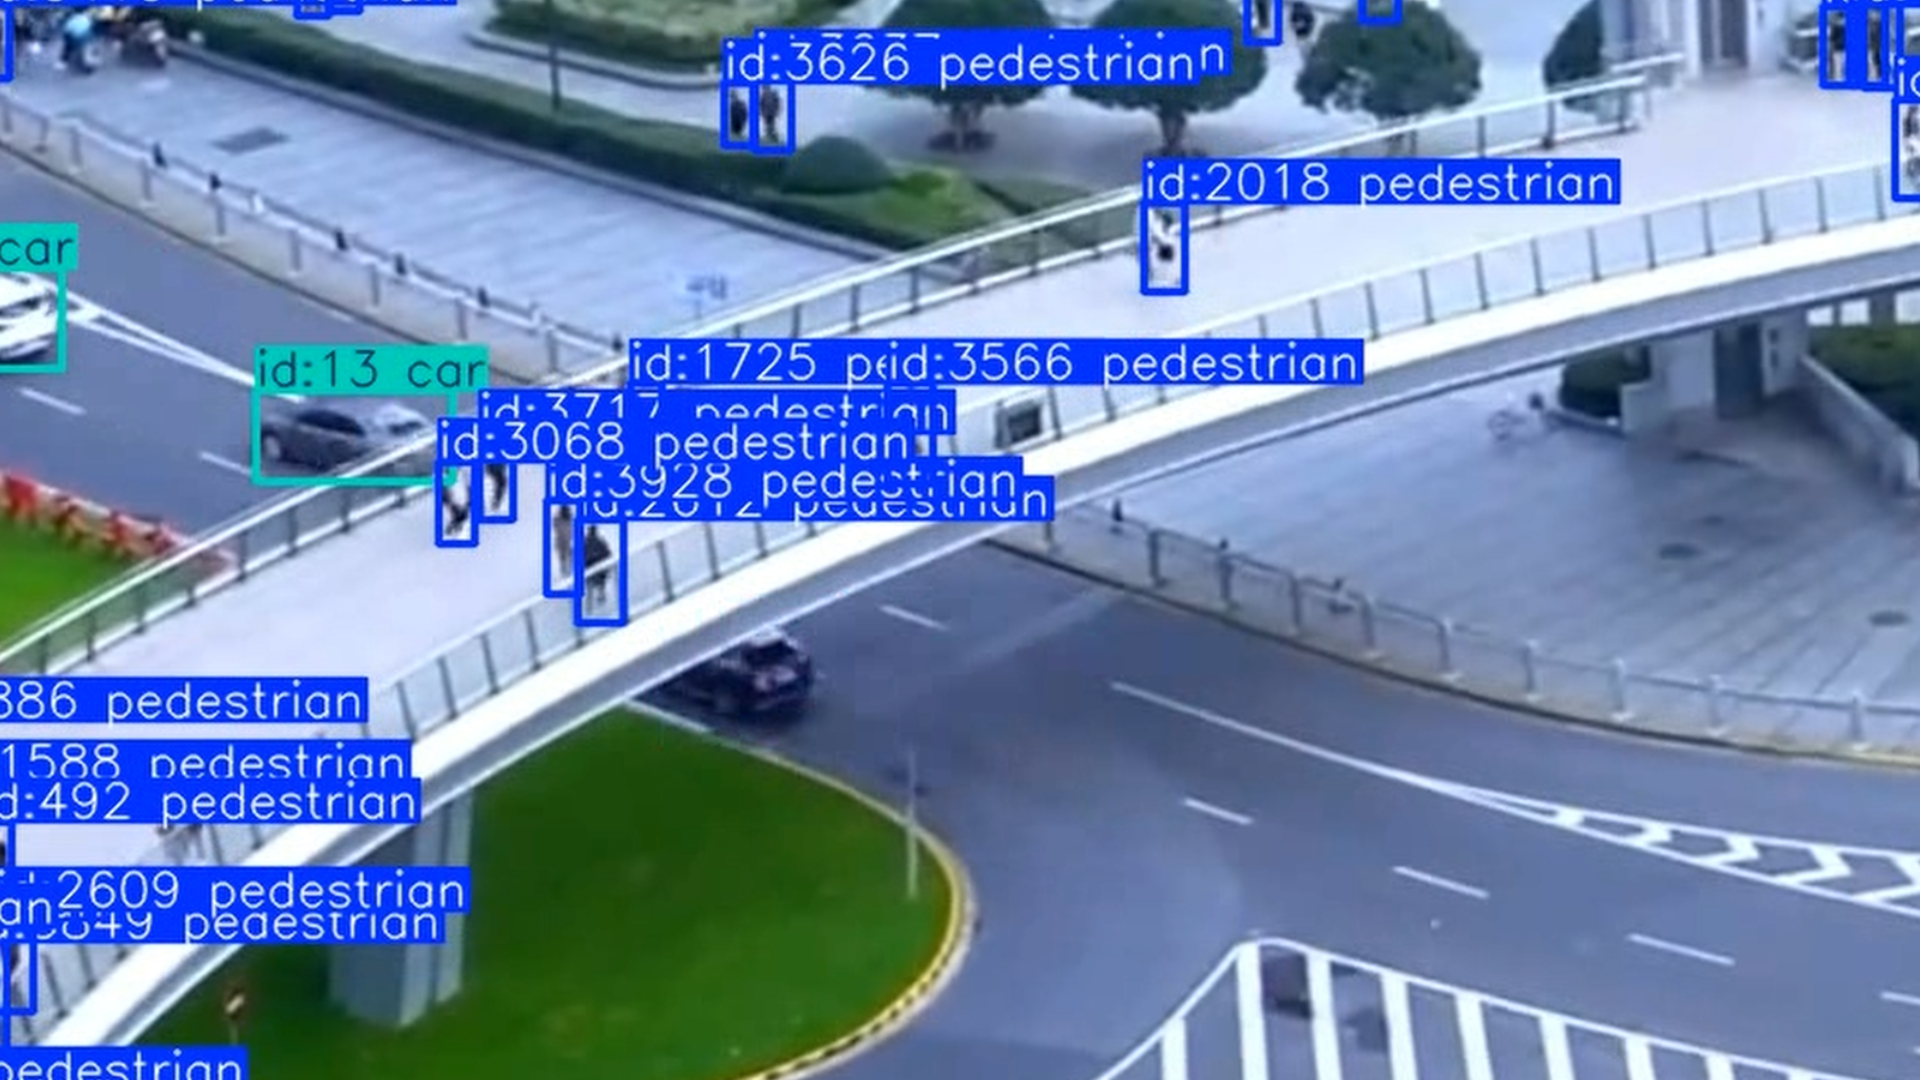
\includegraphics[width=0.24\textwidth]{figures/task2/Frames/Frame 93.jpg}

    {\hspace{0.07\linewidth}\small Frame 90 \hfill Frame 91 \hfill Frame 92 \hfill Frame 93\hspace{0.07\linewidth}}

    \caption{Vehicle passing underneath the pedestrian overpass with environmental occlusion.}
    \label{fig:vehicle_occlusion}
\end{figure}

\subsubsection{ByteTrack Recovery Mechanism}
In both scenarios, the recovery of the original IDs is enabled by the trajectory prediction and association mechanism of ByteTrack. During temporary detection failure, the tracker continues estimating object trajectories using Kalman filtering. Once valid detections reappear, ByteTrack performs data association between predicted trajectories and current detections using the Hungarian matching algorithm. Since the target motion remains sufficiently continuous and the occlusion duration does not exceed the tracker persistence limit, the tracker successfully restores the original identities instead of assigning new IDs.
